\documentclass[12pt]{article}
%% Language and font encodings
\usepackage[english]{babel}
% \usepackage[utf8x]{inputenc}
\usepackage[T1]{fontenc}


%% Sets page size and margins
% \usepackage[letterpaper,top=3cm,bottom=2cm,left=3cm,right=3cm,marginparwidth=1.75cm]{geometry}
\usepackage[margin=1.3in]{geometry}


%% Spacing
\usepackage{setspace}
% \doublespacing
 \onehalfspacing % ASI ESTABA 

%% Useful packages
\usepackage{amsmath}
\usepackage{amssymb}
\let\Bbbk\relax
\usepackage{newtxtext,newtxmath}
\usepackage{adjustbox}
\usepackage{graphicx}
\usepackage{rotating}

% \usepackage[colorinlistoftodos]{todonotes} activate for side notes

\usepackage[colorlinks=true, allcolors=blue]{hyperref}
\let\openbox\relax
\usepackage{amsthm}
\usepackage{lscape}
\usepackage{thmtools}
\usepackage{thm-restate}

\usepackage{color,soul}
\usepackage{xcolor}

\usepackage{tikz}

%% for tables
\usepackage{booktabs}
\usepackage{booktabs, caption}
\usepackage{tabularx}
\usepackage{array}
\newcolumntype{P}[1]{>{\centering\arraybackslash}p{#1}}
\newcolumntype{M}[1]{>{\centering\arraybackslash}m{#1}}
\usepackage[flushleft]{threeparttable}
\usepackage{multirow}
\usepackage{siunitx}
\usepackage{changepage}
%\usepackage{pdflscape}
% for placing figures
\usepackage{float}
\usepackage{placeins}
\usepackage{rotating} % For rotating tables
%\usepackage[nolists,tablesfirst]{endfloat}
%\usepackage{caption,rotating}
% citations
\usepackage{natbib}
% \bibliographystyle{abbrv}
%\bibliographystyle{abbrvnat}
\setcitestyle{authoryear,open={(},close={)}}
% \setlength{\bibsep}{0.0pt}

% \usepackage{bibspacing}
% \setlength{\bibitemsep}{.2\baselineskip plus .05\baselineskip minus .05\baselineskip}

% appendices
\usepackage[toc,page]{appendix}

% Custom definitions
\def\bmath#1{\mbox{\boldmath$#1$}}
\def\sym#1{\ifmmode^{#1}\else\(^{#1}\)\fi}
\declaretheorem[name=Theorem,numberwithin=section]{theorem}
\declaretheorem[name=Proposition,numberwithin=section]{proposition}
\declaretheorem[name=Lemma,numberwithin=section]{lemma}
\declaretheorem[name=Corollary,numberwithin=section]{corollary}
\declaretheorem[name=Definition,numberwithin=section]{definition}
\declaretheorem[name=Example,numberwithin=section]{example}


\newtheorem{assumption}{Assumption}
\newtheorem{property}{Property}

%for highlighting
\usepackage{soul}

%for including pdfs
\usepackage{pdfpages}

% \usepackage{titling}

% multiple footnotes
% \usepackage[multiple]{footmisc}
 
%  for cases in equations
 \usepackage{mathtools}
 
 % For comments

\newcounter{marginparcounter}
\newcommand{\paulapar}[1]{\stepcounter{marginparcounter}$^{(\roman{marginparcounter})}$\marginpar{\renewcommand{\baselinestretch}{0.8}\scriptsize$^{(\roman{marginparcounter})}$ PA: #1}}
\newcommand{\martinpar}[1]{\stepcounter{marginparcounter}$^{(\roman{marginparcounter})}$\marginpar{\renewcommand{\baselinestretch}{0.8}\scriptsize$^{(\roman{marginparcounter})}$ MS: #1}}
\newcommand{\kristianpar}[1]{\stepcounter{marginparcounter}$^{(\roman{marginparcounter})}$\marginpar{\renewcommand{\baselinestretch}{0.8}\scriptsize$^{(\roman{marginparcounter})}$ KLV: #1}}
 

\usepackage{graphicx} % for \includegraphics
\usepackage{subcaption} % for subfigure
\usepackage{rotating} % for sidewaystable and sidewaysfigure

%%%AEJ-Micro wants roman numerals for sections and capital letters for subsections
%\renewcommand{\thesection}{\Roman{section}}
\renewcommand\thesection{\Roman{section}}
\renewcommand\thesubsection{\Alph{subsection}}


\title{Flow Trading: A Laboratory Test}

\author{
  Daniel Friedman\thanks{
  University of Essex and University of California Santa Cruz. Email: dan@ucsc.edu} 
\and
  Yilin Li\thanks{
  University of California Santa Cruz. Email: yli568@ucsc.edu} 
\and
  Kristian L\'opez Vargas\thanks{
  University of California Santa Cruz. Email: klopezva@ucsc.edu}
  \thanks{
We are grateful to Elena Asparuova, Peter Bossaerts, Eric Budish, Peter Cramton, John Duffy,  Grace Gu, Galina Hale, Juergen Huber, Julian Martinez Iriarte, Heinrich Nax, Stephan Palan,  Jean Paul Rabanal, Brett Williams and  Andreas Ziegler
for helpful comments,  
and to audiences at the Theory and Experiments in Monetary Economics (TEME) Conference 2022 at GMU, the 2023 Experimental Finance Conference in Sofia, Chapman University Economics Workshop in April 2024, and the University of Queensland e-seminar in August 2024.
We are indebted to Zhangxi Lin for the software developed for this experiment. We
gratefully acknowledge funding from the UCSC Center for Analytical Finance, the Department of Economics at UCSC, and the European Research Council (ERC) under the European Union’s Horizon 2020 research and innovation programme (grant agreement No 741409).}
}

\date{August 27, 2024}

\begin{document}

\maketitle

\vspace{-.4in}
\begin{abstract}
\begin{singlespace}
The Flow Market format, proposed by \cite{Kyle2017}, is intended to improve on the Continuous Double Auction (CDA) format currently used in most financial markets worldwide. 
The Flow Market format enables traders to specify, as a function of current price, a finite speed (in shares per second) at which they will buy or sell shares. 
This new format is intended to protect traders from exploitation by high-frequency trading (HFT) firms and to effectively shred orders to mitigate adverse price impact. 
We report a human participants experiment comparing the Flow and CDA formats in a simple laboratory environment.
We find that the Flow format reduces price volatility, enhances liquidity and encourages traders to send fewer and larger orders, indicating more effective shredding. The two formats do not significantly differ in terms of price and allocative efficiency in our environment. %However, the Flow Market leads to lower price volatility and perhaps to smaller asymmetries in profits. 
Total trade volume is lower under the Flow Market than under CDA, but the gap narrows in later periods as traders begin to master the mechanics of the Flow format. 
% Our evidence suggests that the flow format initially poses a more complex trading environment. Still, agents learn to trade under such rules, leading to similar efficiency metrics with reduced volatility \hl{and ...}.
Our findings provide initial insights into the Flow format and hint of its potential to improve financial market performance.

\noindent\textit{JEL classification}: C91, D44, D47, G14.

\noindent \textit{Keywords}: Market Design, Continuous Double Auction, Continuous Limit Order Book, Flow Trading, Financial Markets, Laboratory Experiments, High-Frequency Trading, Price Impact, Experimental Finance.

\end{singlespace}
\end{abstract}

%%%%%%%%%%%%%%%%%%%%%%%%%%%%%%%%%%%%%%%%%%%%%%%% 
% \pagebreak
%  \tableofcontents



%%%%%%%%%%%%%%%%%%%%%%%% INTRODUCTION
\newpage

\section{Introduction} \label{introduction}

We report an empirical study of the Flow market format, first proposed by \cite{Kyle2017} and recently extended by \cite{Budish2023}, that aims to 
correct design flaws in existing financial markets. 
The proposed new format differs substantially from existing formats,
so it is problematic to extrapolate its performance from existing data. 
We therefore build a simple laboratory environment within which we directly compare trader behavior and market performance under the new format to that under the format that currently dominates financial markets.

That dominant format, the continuous double auction (CDA, also known as the continuous limit order book), is a streamlined electronic version of 20th-century manual centralized markets. In the CDA, traders' buy and sell orders are posted in a dynamic public order book and matched based on price-then-time priority. Order types include market orders, transacted immediately at the best available price, and limit orders, transacted only when they can be matched at the specified price (or better). 

The CDA is called “continuous” because trade can occur at any instant. 
However, under this format, transaction prices and cumulative quantities are discontinuous functions of time. 
Prices are discrete: multiples of a fixed minimum step, called a tick (typically now \$0.01 and \$0.125 in the 20th century). 
Likewise, orders are multiples of a minimum quantity,
typically either 1 share or 100 shares. 
Orders are processed serially, one at a time, as they arrive. 
Orders that don't produce immediate transactions are stored in the order book, forming supply and demand schedules. 
Those schedules are step functions, due to the   discreteness of prices. 
Often two or more different orders are tied at relevant price steps.
Existing CDA formats resolve ties on price in favor orders that arrived earlier, i.e., they use price-then-time priority. 
%Thus the conjunction  of discrete prices with strict price/time priority gives the advantage to traders who are quickest at updating their orders.

It follows that modern telecommunication technology is remarkably consequential for the CDA. Traders   
with the speediest communication links (generally referred to as  high-frequency traders or HFTs)
can exploit the CDA format by being first in line at a competitive price. Since prices move in discrete steps, it is hard to outcompete a trader with a speed advantage of even a fraction of a millisecond. 
HFTs can react faster to new information and, before slower traders can respond, they can cancel their own orders and pick off stale orders resting in the book. 
Also, firms with superior technology can more effectively ``shred'' their orders, i.e., send sequences of small orders instead of a single large order.
Such firms aim to have smaller price impact and hence more favorable transaction prices and larger trading profits than their lower-tech peers. 

The upshot is that, in recent decades, the CDA format has 
seemed to ``tilt the playing field'' in favor of HFTs and other firms with cutting-edge technology. 
Such a tilt of course raises concerns about market fairness. 
It also
leads to an unproductive ``arms race'' in which firms spend billions of dollars to acquire faster communication and better trading infrastructure than their rivals (\citealp{Budish2015}).
Such investments in speed may impair  effective liquidity, as fast firms cancel orders in the book at the first sign of trouble and slower firms become reluctant to place orders in the book for fear of being picked off \citep{Easly2012}.
The interaction of proprietary fast algorithms may increase price volatility and the risk of  market instability, e.g., flash crashes \citep{aldrich2017flash}.

As noted in the literature survey below, in recent years these perceived problems have provoked a variety of reform proposals, one of which is the Flow market format. 
A Flow market  processes a new type of order, the Continuous Scaled Limit Order (CSLO), which %allows trading at a finite speed within a continuous price range. These orders are defined by five parameters: direction (buy or sell), maximum quantity (\(Q_{\max}\)), a price range between lower (\(P_L\)) and upper (\(P_H\)) limits, and a maximum trading speed (\(U_{\max}\)), in shares per unit of time. CSLOs 
enables traders to more fully express their desired immediacy. 
Traders specify upper and lower price limits $P_U$ and $P_L$ of their price range, and a maximum desired trading speed $U_{\max}$ in shares per second. 
Actual 
%in a richer fashion than standard limit orders in the CDA, since CSLOs 
trading speed, \(U(p(t))\), at time $t$ depends on the current market price, \(p(t)\). Full trading speed,
$U(p(t))=U_{\max}$, is applied at sufficiently favorable prices --- below \(P_L\) for bids and above \(P_H\) for asks. Within the chosen price range, the trading speed for buy orders decreases linearly in $p(t)$, and for sell orders increases linearly.
At less favorable prices outside the trader's chosen range,
$U(p(t))=0$ so the trader stops buying or selling altogether. 

The Flow format is intended to undercut speed advantages --- the upper bound on trading speed allows a HFT to pick off only tiny fractions of orders before slower traders can respond. 
The Flow format may also undercut proprietary order shredding technology, because a finite trading speed in effect automatically  shreds orders finely. 

Despite its potential importance, the Flow format has, to our knowledge, not yet been studied empirically.
A laboratory experiment seems to us an appropriate starting point. 
Holding all else equal, we shall compare human trader behavior and market performance in the continuous double auction (CDA) to that in the  Flow trading format. In our laboratory setting, a single asset is traded on a single exchange, and traders can own or owe hundreds of asset units. 

We induce value for the asset via ``contracts,'' a slight variant of the standard procedure.  
The contracts are of two types: buy contracts, committing the experimenter to repurchase a specified number of shares from the trader at a specified price and time, and sell contracts, a similar commitment to resell shares to the trader. Traders earn profits (cash that they take home at the end of the experiment) to the extent that,
within the allotted time,
they transact at prices more favorable than those specified in their contracts.

This simple laboratory environment allows us to address two primary questions.
(1) Is the Flow format implementable in a way that human traders can understand?
(2) Relative to a standard CDA format, does the automatic internal shredding in the Flow market enable traders to reduce price pressure and the need to manually shred their orders?

More complicated laboratory environments, not explored in the present paper, could investigate  further questions such as whether the Flow format mitigates HFT (or latency arbitrage) problems  and whether
it facilitates trade in multiple inter-related assets.

%The experimental design utilized a between-group approach, with 80 participants divided into 40 per market format across five groups of eight traders. Each market session consisted of 20 trading periods, lasting two minutes each, with eight traders per market. The participants were evenly split between receiving buy and sell contracts. The 20 trading periods were split into five blocks, each containing four periods with constant contract settings for repeated underlying demand and supply conditions.  

%We find significant changes in traders' behavior emerging from the possibility of managing order sizes and frequencies more effectively under the Flow format. Specifically, 
The results of our experiment are instructive. 
Traders from our undergraduate subject pool seem able to master our implementation of the Flow market format, although perhaps not as quickly as the CDA format. 
The automatic order shredding in the Flow market format leads to substantially fewer orders placed (roughly half as many as in the CDA) but substantially larger orders (on average roughly 50 \% larger than in the CDA). 
Despite that apparent improvement in order management, the total traded volume in the Flow Market is lower than in the CDA, but the gap narrows in later trading periods.
Even in our simple laboratory environment, which offers little opportunity for picking off stale orders in the order book, price volatility is only about half as large in the  Flow Market as in the CDA. 
We introduce a ``price pressure index'' that indicates that the Flow market on average is far more liquid than the CDA.
Our measures of market efficiency do not differ significantly between the two formats.
 

Our paper contributes to the literature on design alternatives to the CDA (or continuous limit order book)  format in the presence of heterogeneous access to technology and high-frequency trading firms. 
Frequent batch auctions (FBA, proposed by \citealp{Budish2015}) gather orders over fixed, short time intervals and clear them in a call auctions at the end of each interval. To the extent that the batching time interval exceeds HFT traders' speed advantage, speed rents are diluted. \cite{Aldrich2019} use laboratory experiments to
compare CDA and FBA formats in terms of predatory trading behaviors, technology investment, transaction costs, and volatility. They find that FBA indeed reduces predatory behaviors, diminishes the investment in socially inefficient speed-enhancing technologies, and lowers transaction costs and volatility compared to CDA. \cite{Haas2021} also studied this matter theoretically and found that relative to continuous-time trading, FBAs reduce HFT informational rents.

\cite{Aldrich2022} examine an alternative to the standard CDA that features delayed messaging with order pegging.  %They explore the potential of using intentional messaging delays in financial markets to counteract the advantages of high-frequency traders over traditional traders. 
Their model and empirical analysis show that, with immediate price updating of midpoint pegs, a brief delay in processing new orders  can safeguard slower traders' orders from being exploited by HFTs. However, the message delay introduces additional transaction costs and queuing costs. 

\cite{brolley2023} propose micro-burst fees that target the economic incentives fueling HFT. By imposing a fee on liquidity-taking orders during periods of high message traffic, the proposed format aims to deter latency arbitrage, improve market liquidity, and increase exchange revenues beyond what traditional colocation fees offer. Their theoretical model shows that such fees can reduce the incentive for HFTs to engage in predatory practices. 
\cite{Degryse2022} explore the implications of different order execution rules, such as price-time (PT) priority versus price-broker-time (PBT) priority, where the latter includes broker identity in the priority scheme. Employing both theoretical and empirical analysis, the authors model investor behavior under these priority regimes. They find that the preferred design, PT or PBT, depends on the size of the price tick relative to the dispersion of investors' valuations. 

The Flow market format was first proposed by  \cite{Kyle2017}, as a means of internalizing order shredding and reducing price pressure. They also noted its potential for mitigating problems associated with latency arbitrage.
\cite{Budish2023} propose a multi-market trading institution that combines features of Flow markets (continuous scaled limit orders, generalized to cover portfolios of assets) with those of FBAs (batching orders and clearing them at the end of each short time interval). 
They prove the existence and uniqueness of clearing prices, and demonstrate computational feasibility.

This recent literature is mainly theoretical. 
Empirical assessment of the proposed designs is challenging because most of those designs have never been implemented outside the lab, and so observed data are sparse and indirect.\footnote{
The main exception, as noted in \cite{Aldrich2022}, is that pegs and delayed messaging have been used for several years by IEX and its competitors.}$^,$\footnote{As noted in \cite{cramton2017electricity}, and \cite{cramton2024forward}, 
% [\textcolor{red}{cite Cramton} (2017) and Cramton et al. (2024) [the first entry at cramton.umd.edu/electricity],
in the last 20 years, wholesale electricity markets have employed a (less) frequent batch auction that clears every hour in most cases, although there are some that clear every 15 minutes and a few with a batching interval as short as 4 
seconds.}$^,$\footnote{Other laboratory market studies are more distantly related. \citep{brewer2002behavioral} 
introduce ``continually refreshed supply and demand,'' in which traders who just transacted are immediately replaced by new traders with the same induced preferences --- a different interpretation of flow supply and demand that could be implemented via our contract procedures. 
\cite{mccabe1993designing} test a novel market institution called UPDA that, like the CDA, continuously updates the clearing price as new limit orders arrive but, like the Call market, only executes trades at a uniform (final clearing) price at the end of the trading period.}

It seems appropriate to us that an empirical first step for many of these proposed designs is a carefully designed laboratory experiment parallel to the one we report here for the Flow format.
The logic is the same as for testing new aerodynamic designs in a wind tunnel before trying them in the air, or for testing spectrum auction designs in the laboratory before conducting the actual multi-billion dollar auctions (e.g., \cite{Binmore2002}).

The rest of the paper is organized as follows: Section \ref{Experiment} presents our laboratory procedures. Section \ref{results} presents the results, and Section \ref{conclusion} summarizes the conclusions and discusses possible future research. Appendix A lays out the logic and implementation details for our new price pressure index, Appendix B includes supplementary data analysis, and Appendix C is a copy of instructions to human participants.




%%%%%%%%%%%%%%%%%%%%%%%%%%%%%%%%%%%%%%%%%%%%%%%%%%%%%%%%%%%%
\section{Experiment}
\label{Experiment}

After presenting the laboratory environment in Section \ref{sect:contracts}, we will describe the two market formats and their laboratory implementation in Section \ref{sect:formatimp}.
Section \ref{sect:design} lays out the experiment design, which facilitates head-to-head comparisons of the two formats. 
Section \ref{sect:metricHyps} presents the metrics that we shall use to compare the two formats as well as the hypotheses that we will test.
\subsection{Simple Contract Environment}\label{sect:contracts}

In our experiment, a single asset is traded on a single exchange, and traders can own or owe multiple units (``shares'') of this asset. All prices are expressed in Experimental Currency Units (ECUs).
Profits in ECUs are converted into US Dollars and paid to participants at the end of the session.

We implement a slightly non-standard induced value environment that features  \textit{buy and sell contracts}. 
A buy contract is a commitment from the experimenter to buy from the trader a specified number of shares at a specified price at a specified time later in the trading period. 
For example, the contract ``Buy 300 shares at price  14 ECUs in 80 seconds" means that 80 seconds from now, the experimenter will buy up to 300 shares from the trader's inventory at a price of 14 ECUs per share. If the trader holds no more than 300 units, the experimenter will purchase her entire inventory. 
Likewise, the contract ``Sell 400 shares at a price of 13 ECUs in 90 seconds" means that, in 90 seconds, the experimenter will sell to the trader up to 400 shares at the price of 13 ECUs per share. If the trader is short (owes) only 350 shares, then the experimenter will sell just 350 units to this trader at that price. 

Contracts induce values and create incentives to trade that are similar to classic double auction procedures.
For traders with a buy contract, it is profitable to buy up to the specified number of shares from other traders at prices lower than the contract price before the specified time. 
Similarly, for traders with a sell contract, it is profitable to sell shares at prices higher than the contract price before the specified time. 
Buyers earn the difference between the contract price and the average buying price on each share the experimenter purchases from their  inventory, and similarly, sellers  earn the difference between their average selling price and the contract price. 
Timing is quite flexible --- each contract can arrive and can expire at any times chosen by the experimenter. 

Traders can also profit from trading outside the contract. For example, a trader with a buy contract at 10 ECU per share could profitably sell part of her inventory to another trader willing to pay a price above 10. 

Two differences from standard induced-value asset market environments are worth noting. First, among other things, our study aims to measure how order fragmentation (``shredding'') differs between the two formats. For that purpose, it is necessary to have a finely divisible asset, e.g., to endow traders with hundreds of asset units rather than just one or two units.  
Second, contracts  have flexible arrival and expiration times, which enables the experimenter to manipulate the urgency of trading and to create information events (shifting supply or demand) in the middle of a trading period. However, in the current paper, for the sake of simplicity, each period we give each trader only a single contract at the beginning of the trading period with expiration very near the end of the trading period. 

% \textcolor{red}{Contracts \textbf{are} induced preferences, for multiple (or essentially divisible) units, and potentially are more flexible in terms of timing.
% We need to remind ourselves why we chose this environment (other than it seemed to be what Pete Kyle had in mind) and say a word about that in our writeup.
% Here's what I can recall. (a) trading a single indivisible unit is at best awkward in a flow market, and arguably contradictory. (b) immediacy issues are central to the viability of flow markets, so we need the means to address them in future work. (c) Brett's term paper of about 4 or 5 years ago tried to find close analogues of an ordinary CDA order and had difficulty doing so in the standard environment.}
%Within the framework of these incentives to trade using contracts, our paper studies two different market formats, the continuous double auction (CDA), and the flow trading format (FLOW), and, in particular, the differences in traders' behavior and market performance between these two formats. 

\subsection{Market Formats}\label{sect:formatimp}
In our simple contract environment we compare the performance of two market formats. 

\noindent
\textbf{CDA format.}
The Continuous Double Auction format, also known as the \textit{continuous limit order book}, is designed to process standard limit orders.
These orders are defined by three parameters: a buy-sell indicator, a limit quantity ($Q_{\max}>0
$), and a limit price ($P>0$). A limit order expresses a trader's commitment to buy or sell up to the specified quantity of shares at the specified price or better.

At the core of an exchange operating under CDA is the \textit{order book}, a dynamic repository that prioritizes all pending limit orders lexicographically by their price and then by their submission time. That is, buy orders (i.e., bids) are arranged from the highest to the lowest price; sell orders (i.e., asks) are ordered from the lowest to the highest price. The book prioritizes orders at the same price according to the time of order submission, with earlier orders receiving precedence over later ones. The difference between the lowest ask and the highest bid is called the \textit{spread}.

When a new limit order arrives at a price that matches (or improves) the best available contra-side price, it triggers immediate execution at the contra-side price. 
The executed quantity is the lesser of the quantities specified in the matched buy and sell orders. 
In this case, we say that the arriving order has crossed the market. 
The executed quantity is removed from the order book, and the buyer and seller's cash and inventory are updated to reflect the completed trade.\footnote{
What happens when the arriving order specifies a larger quantity than the best contraside order? 
Then the remainder of the arriving order is treated as a newly arriving order and immeditately executes against the best remaining contra-side order if it matches or improves on the arriving order's price. This process applies recursively.} 
If, instead, the new order does not cross the market, it is stored on its own side of the order book according to the usual price-time priority.


% \textcolor{red}{Yilin, Kristian, this description doesn't say what happens if a large new limit order crosses multiple orders in the book, perhaps at different prices.
% How does your CDA algorithm deal with this? Presumably it rips thru the book (with older booked orders executing first at any price) until either the new order quantity is exhausted, or else the order book is exhausted at better prices and the residual new order is entered in the book. }

% Hi Dan. I added this paragraph. Let me know what you think. 

%If an order arrives and is large relative to the quantity availability at each price level on the other side of the market, CDA sequentially executes the new order against available limit orders, prioritizing them first by price and then by their entry time into the order book. That is, the mechanism first exhausts the available quantities at the best price on the contra side and continues to the second best price and so on until either the entirety of the large order is fulfilled or the order book runs out of available orders on the contra side to match it with. At this point, any remaining quantity of the new order is added to the order book at the stipulated price. The concept of \textit{price impact} is precisely connected to this process. Price impact refers to the change in market price resulting from the execution of a trade. When a large order rips through the book, its execution across multiple price levels can significantly move the market price, having a substantial price impact. This is because the large order consumes available liquidity at the best prices but then moves onto worse prices. 
% The initial orders are executed at prices close to the current market price. Still, as the order matches deeper into the book, it encounters orders placed at less favorable prices, leading to a more pronounced change in the market price. 

\bigskip
\noindent
\textbf{CDA User Interface.}
As illustrated 
in Panel (a) of Figure \ref{fig:exp_interfaces}, human traders in our CDA markets have a screen display that enables them to operate on both sides of the market.
The top middle box of their screen
(labeled Your Input) allows the trader to set and submit limit orders. The horizontal axis denotes the quantity of shares, and the vertical axis denotes prices in ECUs per share. To set a \textit{buy} order, the trader drags the blue dot inside the grid to set the desired price and the quantity. 
Then the trader submits the order by clicking the blue ``Send Buy" button (which then becomes a ``Cancel Buy'' button, as shown). 
%The blue-line segments graphically describe her buy order. 
Similarly, the trader sets a \textit{sell} order by dragging the red square inside the grid to the desired price and the quantity and submits it by clicking the red  ``Send Sell" button. 
These submitted orders appear as  text in the Active Orders table on the left side of the screen. 
To submit a new buy (sell) order, the trader must cancel her active buy (sell) order and then create and submit a new one. 

The top-right box (labeled Market) displays the current limit order book, updated with imperceptible delay after each order 
(include the trader's own orders) is submitted and processed. 
The blue curve (step function) 
is the market demand, and the red is the market supply. Their intersection determines the instantaneous trading price and the traded quantity;
the arrival of a crossing order immediately generates a trade.
(Almost always, demand and supply cross each other along the vertical axis $(q=0)$ representing the CDA's most common state where the best bid is below the best ask; only when an order arrives at or beyond the best contra-side price do the supply and demand cross for an instant and generate a trade.) 
The larger green dots on the graph show the price and quantity of the more recent trades.

The bottom-right box on the trader's screen tracks her inventory and cash balance within each trading period. 
The bottom middle box tracks her projected profit, i.e., what her earnings that period would be if her active contract were to expire and the period were to end immediately. 
The top left table shows her active contracts; in our simple environment, it shows the contract she received right after the start of the trading period. 
As noted earlier, the table below describes the trader's active (unexecuted) orders, and 
the table below displays her orders that have already been executed earlier in the period. 
The bottom-left table in our simple environment remains blank until the end of the period, when the contract expires. At that time, it shows what portion of the trader's previously active contract was filled. 

\bigskip
\noindent
\textbf{Flow format.}
The Flow market processes  \textit{Continuous Scaled Limit Orders}, % CSLOs enable a continuous price range for the flow trading of shares. 
each characterized by five parameters: a directional indicator specifying buy or sell, a maximum quantity (\(Q_{\max}\)) to be traded, a price range defined by lower (\(P_L\)) and upper (\(P_H\)) bounds with \(0<P_L < P_H\), and a maximum trading speed (\(U_{\max}\)), measured in shares per second. This framework allows traders to express their willingness to transact up to a specified quantity within a defined price range at a speed that does not exceed \(U_{\max}\).

CSLOs enable traders to express the trading speed \(U(p(t))\) at which they wish to trade as a function of the current market clearing price \(p(t)\). 
Full speed (\(U_{\max}\)) is maintained when the market price is at or below the lower price threshold (\(P_L\)) for buy orders, or above the upper price threshold (\(P_H\)) for sell orders, i.e., when prices are sufficiently favorable to the trader.
Within the price range (\(P_L \leq p(t) \leq P_H\)), the trading speed decreases linearly with price for buy orders and increases linearly for sell orders. Thus trading speed diminishes at less favorable prices. 
%The linear interpolation ensures that the execution rate diminishes as prices approach the less favorable end of the specified range, reflecting a trader's diminishing willingness to trade as prices move away from the trader's best conditions. 
Trading ceases (\(U(p(t)) = 0\)) when price $p(t)$ falls outside the favorable range—i.e., above \(P_H\) for buy orders or below \(P_L\) for sell orders. Thus the trader withdraws from the market when the clearing price lies outside her acceptable price range. 
The trader also withdraws from the market when her order is fully executed, i.e., when the accumulated flow reaches her specified total quantity \(Q_{\max}\).

To spell this out, let $p(t)$ be the clearing price. If the trader's CSLO specifies maximum speed $U_{\max}$, price range $(P_L , P_U)$ and direction buy ($d$), then her trading speed is
\begin{equation}\label{eq:flowd}
U_{d}(p(t)) = \begin{cases}
U_{\max} & \text{if } p(t) < P_L \\
\frac{P_H - p(t)}{P_H - P_L} U_{\max} & \text{if } P_L \leq p(t) \leq P_H \\
0 & \text{if } p(t) > P_H
\end{cases}
\end{equation}
If instead the direction is sell ($s$),
then it is
\begin{equation}\label{eq:flows}
U_s(p(t)) = \begin{cases}
	U_{\max} & \text{if } p(t) > P_H\\
	\frac{p(t) - P_L}{P_H - P_L} U_{\max} & \text{if } P_L \leq p(t) \leq P_H \\
	0 & \text{if } p(t) < P_L 
\end{cases}
\end{equation}

Summing the expressions (\ref{eq:flowd}) and (\ref{eq:flows})
across traders with active orders, one obtains flow demand and supply $D(t)$ and $S(t)$ that are strictly monotone piece-wise linear functions of the price at any given point in time. 
As illustrated in Figure \ref{fig:snd}, the 
intersection ($U(t), p(t)$), therefore uniquely determines the instantaneous clearing price and the overall transaction rate.
 Individual trading speeds are, in turn, dictated by each trader's specific flow demand or supply curve evaluated at the clearing price. 

% a / b, c / d, (a + c) / (b + d)
 
\begin{figure}[H]
    \centering
    \caption{Clearing price example.}
    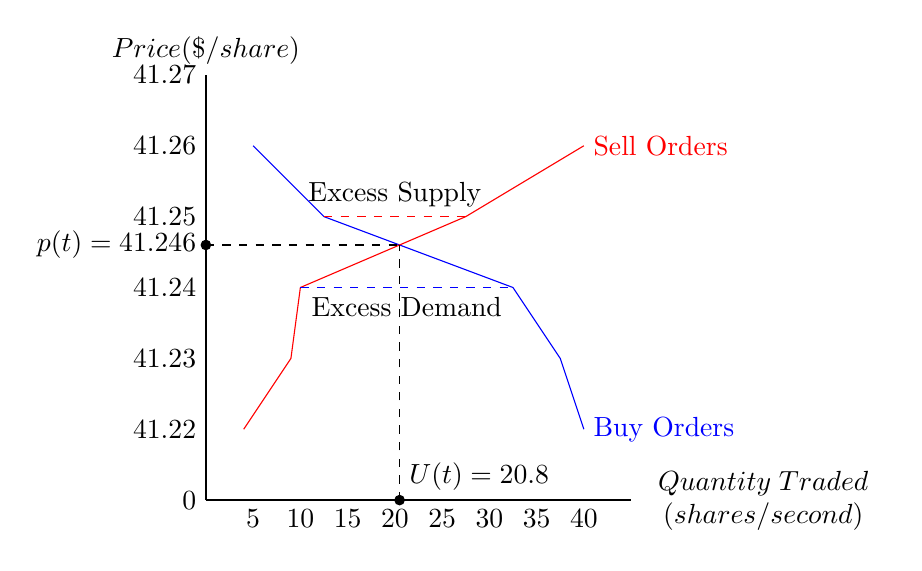
\begin{tikzpicture}[scale=0.6]
        \draw[thick,-] (0,0) -- (0,9) node[above]{$Price (\$/share)$};
        \draw[thick,-] (0,0)--(9,0) node[right]{\begin{tabular}{c}
             $Quantity \; Traded$ \\
             $(shares/second)$
        \end{tabular}};
        \node[left] at (0,1.5) {$41.22$};
        \node[left] at (0,3.0) {$41.23$};
        \node[left] at (0,4.5) {$41.24$};
        \node[left] at (0,6.0) {$41.25$};
        \node[left] at (0,7.5) {$41.26$};
        \node[left] at (0,9.0) {$41.27$};
        \node[below] at (1,0) {$5$};
        \node[below] at (2,0) {$10$};
        \node[below] at (3,0) {$15$};
        \node[below] at (4,0) {$20$};
        \node[below] at (5,0) {$25$};
        \node[below] at (6,0) {$30$};
        \node[below] at (7,0) {$35$};
        \node[below] at (8,0) {$40$};
        \node[left] at (0,0) {$0$};
        \draw[blue,solid] (1,7.5) -- (2.5,6.0) -- (6.5,4.5) -- (7.5,3) -- (8,1.5) node[right]{Buy Orders} ;
        \draw[red,solid] (0.8,1.5) -- (1.8,3) -- (2,4.5) -- (5.5,6) -- (8,7.5) node[right]{Sell Orders};
        \draw[red,dashed] (2.5,6.0) -- (5.5,6.0);
        \draw[blue,dashed] (2,4.5) -- (6.5,4.5);
        \node[black,above] at (4,6.0) {Excess Supply};
        \node[black,below] at (4.25,4.5) {Excess Demand};
        \draw[dashed] (4.1,0) -- (4.1,5.4);
        \draw[dashed] (0,5.4) -- (4.1,5.4);
        \node[above right] at (4.1,0) {$U(t)=20.8$};
        \draw[fill] (4.1,0) circle [radius=.1];
        \node[left] at (0,5.4) {$p(t)=41.246$};
        \draw[fill] (0,5.4) circle [radius=.1];
    \end{tikzpicture} \\
    \raggedright \footnotesize Note: Excess supply = 28 - 12 = 16 shares at \$41.25 and excess demand = 34 - 10 = 24 shares at the next lower tick, \$41.24, so the clearing price is $\frac{41.24 ^* 16 \ + \ 41.25 ^* 24}{16 \ + \ 24}$ = \$41.246.
    \label{fig:snd}
\end{figure}

The flow format enables traders to finely tailor their market engagement. Their chosen CSLOs reflect not only their target prices but also their urgency of trading. It is not hard to see that the impact a CSLO has on clearing price is reduced when a trader reduces her $U_{\max}$ or expands the width $P_U- P_L$ of her acceptable price range.  

\bigskip
\noindent
\textbf{FLOW User Interface.} 
The software and interface for the Flow market is analogous to that of the CDA market. 
Figure \ref{fig:exp_interfaces}(b) shows one trader's FLOW trading screen.  The trader sets and submits buy and sell orders in the top-middle box (titled ``Your Input''). The horizontal axis denotes \textit{rate} in shares per second, and the vertical axis denotes prices in ECUs per share. 
The trader sets a \textit{buy} order by moving the blue dot along the vertical axis to set the high price and dragging the blue square anywhere inside the grid to set the low price and the maximum rate. 
Then she enters the total number of shares she wants to buy in the box next to the ``Send Buy" blue button and submits it by clicking that button. The blue-line segments graphically describe her buy order. %, as shown in Figure \ref{fig:exp_interfaces} panel (b). 
Likewise, she sets a \textit{sell} order by moving the red dot along the vertical axis to set the low price and dragging the red square anywhere inside the grid to set the high price and the maximum rate. Then, she enters the total number of shares she wants to sell in the box next to the ``Send Sell" red button and submits it by clicking that button. She can submit a new order at any time by canceling her active orders on the same side of the market and then creating a new order. 

The trader sees the market supply (the blue piecewise linear curve) and demand (red) in the top-right Market box. Their intersection determines the clearing price $p(t)$ and the aggregate clearing rate $q(t)$. The green horizontal line at height $p(t)$ in the Market diagram extends into the \textit{Your Input} box and indicates the current market price. The x-coordinate of the intersection of this line and the trader's order indicates the trader's current trading speed. The column of tables on the left side and the bottom boxes (projected profits, inventory, and cash) of the FLOW interface parallel those in the CDA interface.  


% \newpage
\begin{figure}
    \centering
    \caption{Experiment Interfaces}
    \begin{subfigure}[b]{\linewidth}
        \centering
        
\includegraphics[width=0.9\linewidth]{figures/cda_ui.png}
        \caption{CDA Format}
        \label{fig:cda_ui}
    \end{subfigure}
    \begin{subfigure}[b]{\linewidth}
        \centering
        
\includegraphics[width=0.9\linewidth]{figures/flow_ui.png}
        \caption{FLOW Format}
        \label{fig:flow_ui}
    \end{subfigure}
    \label{fig:exp_interfaces}
\end{figure}
% \newpage

\subsection{Implementation}\label{sect:design}

We implemented a between-group design. We deployed five market sessions (or groups) with the CDA format and five with the Flow format. Each market consisted of eight traders, interacting in 20 trading periods, each lasting two minutes. 
%That is, each CDA session has a identical twin Flow session with the same pattern of contract assignments, blocks, etc. as detailed below. 
At the start of each trading period of a market,  four traders receive a single buy contract and four receive a single sell contract. %as each period starts. 
As mentioned above, %buy and sell contracts are analogous to induced values and costs in standard market experiments. In particular, 
a buy (sell) contract is a commitment from the experimenter to buy (sell) up to $Q_{\textit{contract}}$ units at price $p_{\textit{contract}}$ at the specified expiration time, here at the end of the trading period. % of the contract (all expiration times were set near the end of the trading period). \


We divided the 20 trading periods into five blocks of four consecutive periods each. 
The four periods within the block have the same contract configuration, i.e., the induced demand and supply curves repeat, and so do the quantity and price of equilibrium. 
Such stationary repetition is intended to give traders the opportunity to discover equilibrium.

The contract configuration changes when the next block begins. 
The intention is to challenge the market to track a shifting equilibrium price and quantity.
We use the three different contract configurations depicted in Figure \ref{fig:3contract_configs_new}.
Configurations (a), (b) and (c) are used in Blocks one, two and three respectively.
Block four repeats the configuration of Block two, and Block five repeats that of Block one. 
The blue staircases in the Figure represent the buy contracts, sorted to form the induced demand curve, and the red supply curve similarly represents the sell contracts. 
Each contract assigned to an individual trader is a step (a flat line segment) on either demand or supply curve. 
Contract information is private: each trader sees her own current contract but not those of other traders.

Within each block, each trader receives the same contract each period. Across blocks, buyers and sellers receive different contracts but keep the same role. The block structure is not announced; traders are simply told that their contracts may (or may not) change from one period to the next. 
% but we assign a new set of contacts as shown in Figure \ref{fig:3contract_configs_new}. 

%%%%% CONTRACT FIGURES %%%%%%%%%

\begin{figure}
    \centering
    % \caption{Contract Configurations}
    \begin{subfigure}[c]{0.33\linewidth}
        \centering
            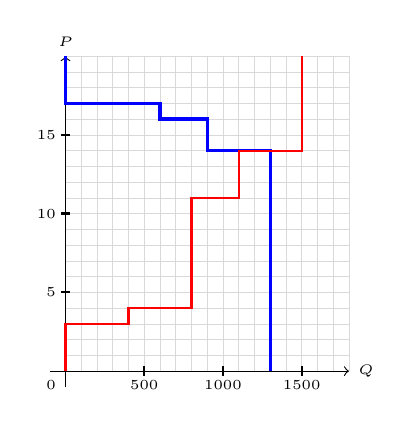
\begin{tikzpicture}[scale=.2]
                % create grid
                \draw[help lines, gray!30] (0,0) grid (18,20);
                
                % Draw axes
                \draw[->] (-1,0) -- (18,0) node[font=\tiny,right] {$Q$};
                \draw[->] (0,-1) -- (0,20) node[font=\tiny,above] {$P$};
              
                % Draw step functions
                \draw[blue, very thick] (0,20) -- (0,17) -- (6,17) -- (6,16) -- (9,16) -- (9,14) - - (13,14) -- (13,0) ;
                \draw[red, thick] (0,0) -- (0,3) -- (4,3) -- (4,4) -- (8,4) -- (8,11) --  (11,11) -- (11,14) -- (15,14) -- (15,20);
                
                % % Add labels
                \node[font=\tiny,below left] at (0,0) {$0$};
                \foreach \x in {5,10,15} {
                  \node[font=\tiny,below] at (\x,0) {$\x00$};
                }
                \foreach \y in {5,10,15} {
                  \node[font=\tiny,left] at (0,\y) {$\y$};
                }
                
                % % Add thicker ticks (Q)
                \draw[black, thick] (5,-0.3) -- (5,0.3);
                \draw[black, thick] (10,-0.3) -- (10,0.3);
                \draw[black, thick] (15,-0.3) -- (15,0.3);

                % % Add thicker ticks (P)
                \draw[black, thick] (-0.3,5) -- (0.3,5);
                \draw[black, thick] (-0.3,10) -- (0.3,10);
                \draw[black, thick] (-0.3,15) -- (0.3,15);
            \end{tikzpicture}
        \subcaption{\tiny Block 1 (T1-T4) \\ and Block 5 (T17-T20)}
    \end{subfigure}%
    \begin{subfigure}[c]{0.33\linewidth}
        \centering
        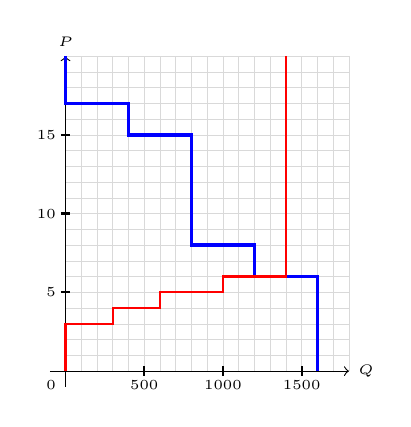
\begin{tikzpicture}[scale=.2]
            % create grid
            \draw[help lines, gray!30] (0,0) grid (18,20);
            
            % Draw axes
            \draw[->] (-1,0) -- (18,0) node[font=\tiny,right] {$Q$};
            \draw[->] (0,-1) -- (0,20) node[font=\tiny,above] {$P$};
          
            % Draw step functions
            \draw[blue, very thick] (0,20) -- (0,17) -- (4,17) -- (4,15) -- (8,15) -- (8,8) -- (12,8) -- (12,6) -- (16,6) -- (16,0);
            \draw[red, thick] (0,0) -- (0,3) -- (3,3) -- (3,4) -- (6,4) -- (6,5) -- (10,5) -- (10,6) -- (14,6) -- (14,20);
            
            % % Add labels
            \node[font=\tiny,below left] at (0,0) {$0$};
            \foreach \x in {5,10,15} {
              \node[font=\tiny,below] at (\x,0) {$\x00$};
            }
            \foreach \y in {5,10,15} {
              \node[font=\tiny,left] at (0,\y) {$\y$};
            }

            % % Add thicker ticks (Q)
            \draw[black, thick] (5,-0.3) -- (5,0.3);
            \draw[black, thick] (10,-0.3) -- (10,0.3);
            \draw[black, thick] (15,-0.3) -- (15,0.3);

            % % Add thicker ticks (P)
            \draw[black, thick] (-0.3,5) -- (0.3,5);
            \draw[black, thick] (-0.3,10) -- (0.3,10);
            \draw[black, thick] (-0.3,15) -- (0.3,15);
        \end{tikzpicture}
        \subcaption{\tiny Block 2 (T5-T8) \\ and Block 4 (T13-T16)}
    \end{subfigure}%
    \begin{subfigure}[c]{0.33\linewidth}
        \centering
        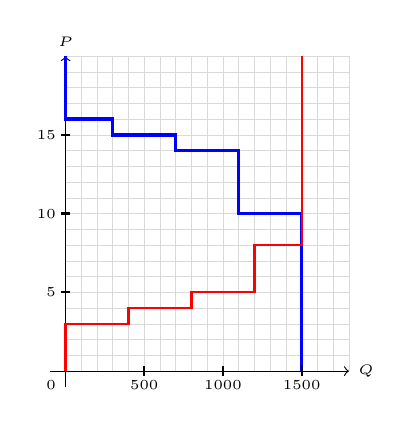
\begin{tikzpicture}[scale=.2]
            % create grid
            \draw[help lines, gray!30] (0,0) grid (18,20);
            
            % Draw axes
            \draw[->] (-1,0) -- (18,0) node[font=\tiny,right] {$Q$};
            \draw[->] (0,-1) -- (0,20) node[font=\tiny,above] {$P$};
          
            % Draw step functions
            \draw[blue, very thick] (0,20) -- (0,16) -- (3,16) -- (3,15) -- (7,15) -- (7,14) -- (11,14) -- (11,10) -- (15,10) -- (15,0);
            \draw[red, thick] (0,0) -- (0,3) -- (4,3) -- (4,4) -- (8,4) -- (8,5) -- (12,5) -- (12,8) -- (15,8) -- (15,20);
            
            % % Add labels
            \node[font=\tiny,below left] at (0,0) {$0$};
            \foreach \x in {5,10,15} {
              \node[font=\tiny,below] at (\x,0) {$\x00$};
            }
            \foreach \y in {5,10,15} {
              \node[font=\tiny,left] at (0,\y) {$\y$};
            }

            % % Add thicker ticks (Q)
            \draw[black, thick] (5,-0.3) -- (5,0.3);
            \draw[black, thick] (10,-0.3) -- (10,0.3);
            \draw[black, thick] (15,-0.3) -- (15,0.3);

            % % Add thicker ticks (P)
            \draw[black, thick] (-0.3,5) -- (0.3,5);
            \draw[black, thick] (-0.3,10) -- (0.3,10);
            \draw[black, thick] (-0.3,15) -- (0.3,15);
        \end{tikzpicture}
        \subcaption{\tiny Block 3 (T9 - T12)}
    \end{subfigure}
    \caption{\textbf{Contract configurations across trading blocks.}  \footnotesize
Vertical axis is price (ECU per share) and horizontal axis is quantity (shares). Each panel plots the step‐function demand schedule (thick blue) and supply schedule (red).  
The intersection of the two schedules determines the competitive‐equilibrium price–quantity pair for that block.  
Panel (a) applies to Blocks 1 (T1–T4) and 5 (T17–T20) of experiment; panel (b) to Blocks 2 (T5–T8) and 4 (T13–T16); panel (c) to Block 3 (T9–T12). }
% \label{fig:contract-configs}
    \label{fig:3contract_configs_new}
\end{figure}

% Yilin please add captions explaining the blocks and the equilibrium values. 

A few comments are in order about the chosen contract configurations. 
First, the rectangular shape of each contract matches the rectangular shape of an ordinary limit order book, in that sense advantaging the CDA. % this facilitates comparable underlying incentives between the two market formats. 
Second, prior experimental evidence 
going back to \cite{friedman1995competitivity} suggests that efficiency in the CDA markets tends to be lower (mainly due to undertrading) when goods are highly divisible; see \cite{angereretal}
for a recent confirmation.
% Investors’ Behaviors and Market Efficiency in Fractionalized Asset Markets by Martin Angerer, Marius Gramlich, and Yilong Xu, unpublished manuscript, University of Liechtenstein, Department Finance & Economics, August 2024
That tendency provides more room for either format to exhibit an efficiency advantage.
Third, the asymmetric surplus in panel (a) of Figure \ref{fig:3contract_configs_new} may lead to slow convergence to competitive equilibrium from below; indeed, excess demand for prices $p \in [11,14)$ below CE is only 1300 - 1100 = 200 shares, while excess supply at $p \in (14, 17]$ above CE is at least 1500 - 900 = 600 shares.
This asymmetry suggests that, in the first block, buyers will tend to make higher profits relative to CE than will sellers.
The second block provides a similar sort of advantage for seller profits, while the third block seems even-handed. As we will see below, those asymmetries indeed seem to influence market dynamics in the corresponding blocks. 
% but it may be that the initial pattern persists.


Experiment instructions were provided on the computer screen and in print; see Appendices \ref{app_instruction_cda} and \ref{app_instruction_flow} for a copy. % Instructions were discussed and piloted (with students and colleagues) to balance clarity and reasonable length.} 
% \footnote{To ensure clarity and understanding of the experiment's rules and objectives, we provided participants with detailed instructions on-screen and paper, supplemented by a video summary. The experiment also included trial periods for participants to familiarize themselves with the interface and market rules. Final payments were based on accumulated wealth, incorporating a fixed participation fee.}
After 15 minutes of reading instructions, a video summary was played with animations and annotations to aid participants' understanding. 
Two 120-second practice periods then familiarized participants with the interface and market rules; questions
were encouraged. 
The 20 actual trading periods then began.
Participants were not allowed to communicate with each other before or during the experiment, nor did they learn the identity or characteristics of other participants.

In between trading periods, each participant viewed a summary screen displaying a profit history of each the previous trading period.
% KLV Should we add a screen in the appendix?
Each participant started each trading period with a zero endowment. 
To simplify their task, they were not allowed to acquire inventory positions 
(short or long) beyond their contract quantity.
As explained in the instructions,
take-home pay consisted of final cash
(after the experimenter fulfilled all contracts) each period summed across all twenty trading periods, and converted to US Dollars at a pre-announced exchange rate of 1000 ECUs = \$1, plus a \$7 participation fee. 
Although it is possible to earn negative ECUs in any one period, this was quite rare, and happened in less than 5\% of periods. 
%4.62\% of the cases (4.88\% in the CDA and 4.37\% in FLOW)
Payments were made privately and averaged \$28.77 per participant %, with a %minimum of \$13.68 and maximum of \$51.99. (std = 
(standard deviation \$8.38).
The experiment software was built on the oTree platform \citep{otree}. Sessions were conducted at the LEEPS Laboratory of the University of California, Santa Cruz and lasted 100 minutes on average. Participants were recruited via LEEPS' ORSEE instance (\hyperlink{https://econlab.ucsc.edu/public/}{econlab.ucsc.edu}; \cite{Greiner2015}).


% \subsection{Hypotheses}
% list the criteria we will use for market quality  --- 
% allocative efficiency, price efficiency, price volatility, profit level and dispersion, ... ---
% and for each criterion offer a hypothesis on which format will be better.

% describe in words how we defined?
%%%%%%%%%%%%%%%%%%%%%%%%%%%%%%%%%%%%%%%%%%%%%%%%%%%%%%%%%%%%%%%%%%%%%%%%%%%%%%%%%%%%%%%%%%%%%%%%%%%%%%%%%%%%%%%%%%%
\subsection{Performance Metrics and Hypotheses}\label{sect:metricHyps}
\label{sec:hypotheses}

To compare the two market formats, we will analyze \textbf{trader behavior} in terms of 
the \textit{number of submitted orders} per trading period, 
the \textit{size of submitted orders}  in shares per order,
the \textit{prices} of the limit orders in the CDA or the continuous scaled limit orders in the Flow format, and
the \textit{maximum trading rate} specified in a CSLO.

We will also analyze \textbf{market performance} using several metrics.
\textit{Absolute Price Change} is defined for each period as the average absolute price difference between adjacent time grid points, $|P_t - P_{t-1}|$. A larger value indicates more erratic prices. 
Our convention on
the (5-second) time grid is described below. %lower price volatility. %\footnote{We define trading intervals at the beginning of the Results section.}
\textit{Price volatility} is defined for each period as the variability of proportional price changes, and is calculated as the standard deviation of $(\ln P_t - \ln P_{t-1})$ across time grid intervals.
%periods and groups. This is another metric of price volatility. 
A new liquidity metric called 
\textit{Price pressure index (PPI)} is defined as the per-share cost of executing a buy-sell round trip of a standard package ($Q^* = 20$ shares),
and is computed within each time grid interval. %in a short time interval ($\Delta t = 5$ seconds). 
A lower PPI indicates greater liquidity and less impact on price; see the Appendix for technical details.  

Other market performance metrics are computed once per period.
\textit{Trade Volume} is defined  as the total quantity of shares traded in a period. An aggregate indicator of market activity, it can be compared to the minimum trading volume required to achieve a competitive equilibrium allocation. An alternative volume metric is \textit{Filled Contract}, the quantity filled by the experimenter when contracts expire; this metric ignores volume due to ``churn,'' e.g.,  traders reselling part of their purchases.
\textit{Informational [in]efficiency} is  defined each period as the mean absolute deviation of transaction price from the  competitive equilibrium price, \( |P_t - P_{\text{CE}}| \). 
Smaller deviations indicate higher informational efficiency, that is, transaction prices that more fully incorporate all private information regarding supply and demand.\footnote{
Thus, in the CE benchmark, \( |P_t - P_{\text{CE}}| \), $|P_t - P_{t-1}|$ and 
$(\ln P_t - \ln P_{t-1})$ are all zero.}
Finally, \textit{Allocative efficiency} is measured as \( \Pi/\Pi_{\text{CE}}\), i.e.,
 realized surplus (the sum of traders' actual profits) as a fraction of potential surplus (the sum of trader profits earned in competitive equilibrium). 
This metric assesses how efficient the market is in extracting potential gains from trade.       


%%%%%%%%%%%%%%%%%%%%%%%%%%%%%%%%%%%%%%
% \vspace{0.5cm}
% \noindent \textit{Hypotheses} \\

Those metrics allow us to formulate the following testable hypotheses. 

%\vspace{0.3cm}
\noindent \textbf{Hypothesis 1: Order shredding.} \textit{Traders will submit a larger number of smaller quantity orders in the CDA format than in the Flow format.} 
%\vspace{0.3cm}

\noindent As discussed earlier, to reduce price impact in the CDA, traders have to shred their orders manually, i.e., to break the overall quantity to be traded into fragments submitted sequentially. By contrast, the Flow format automatically facilitates very fine order shredding since, in each short time interval, only a very limited quantity can be transacted. 
The Flow format can closely reproduce CDA trading and pricing dynamics if traders minimize the separation between $P_L$ and $P_H$ and submit the highest allowed trading rate, ($U_{\text{max}}=30$ shares per second). 
If traders instead modulate their urgency to trade --- by choosing a wide gap between  prices $P_L$ and $P_H$  and/or choosing $U_{\text{max}}$ well below the highest rate allowed by the interface --- then they automatically will greatly reduce price impact even when they submit large orders. Thus, if traders care about price impact,\footnote{\cite{elenaetal} find that, with highly divisible assets, traders in a CDA may shred orders for reasons beyond price impact. 
Specifically, traders may wish to hedge their bets early in the trading period against the possibility of more favorable prices later in the period. Such a diversification motive would not seem very sensitive to the market format, but it suggests that orders may be earlier, fewer and larger in later periods when traders have less uncertainty about price distributions.} 
in the Flow format we should observe fewer but larger orders than in the CDA. 

\vspace{0.3cm}
\noindent \textbf{Hypothesis 2: Volatility.} \textit{Price volatility will be lower with the Flow format than with the CDA.}
%\vspace{0.3cm}

\noindent In the CDA, each transaction is executed at a price determined by a unique bilateral matching of limit orders of a buyer and a seller. This can lead to a wide dispersion of transaction prices within a short time frame. In contrast, the Flow Market operates under a uniform pricing rule — from moment to moment, every trade for every active trader is executed at the same price, until an active order is fully filled or a new order arrives. This uniformity may attenuate transaction price fluctuations, yielding a more stable price path. Hence, we hypothesize that the Flow format brings lower price volatility than the CDA. 


\vspace{0.3cm}
\noindent \textbf{Hypothesis 3: Liquidity.} \textit{ PPI will be lower, i.e., markets will be more liquid, with the Flow format than with the CDA format.}

\noindent 
If the Flow format indeed reduces price volatility and the need to manually shred orders, then it should encourage traders to place larger bids and asks in the order book closer to the current clearing price. Such enhanced liquidity would reduce the round-trip cost of a modest order to buy and resell, i.e., would reduce PPI. 
%The Flow Market is designed to automatically shred orders and execute trades at a more consistent rate relative to the CDA, and at a less volatile uniform price (see previous hypothesis). This should reduce the immediate impact of large orders on prices, leading to lower price pressure. It is then expected that the Flow Market will exhibit a lower Price Pressure Index (PPI). 

\vspace{0.3cm}
\noindent \textbf{Hypothesis 4: Volume.} \textit{The CDA and Flow formats will exhibit similar levels of trade volume. }
%(b) Both will move within each trading block towards the minimum volume that sustains competitive equilibrium.} 
%\vspace{0.3cm}

\noindent There is no obvious reason why the overall trade volume should be larger in one format than the other, so H3 is the natural null hypothesis. We shall also examine whether trade volume in later periods approaches the competitive equilibrium volume. 

\vspace{0.3cm}
\noindent \textbf{Hypothesis 5: Efficiency.} \textit{The CDA and Flow formats will exhibit similar levels of (a) informational and (b) allocative efficiency.} 
%\vspace{0.3cm}

\noindent Again, there is no compelling \textit{a priori} reason to expect one format to be more efficient than the other, either in informational efficiency (prices close to competitive equilibrium) or in allocative efficiency (near exhaustion of gains from trade),\footnote{Note this is not necessarily true in environments such as \cite{Budish2015, Aldrich2019} where equilibrium in the CDA implies socially wasteful investment in technology.}
so H4 is the natural null hypothesis.
% On the other hand, proponents of either format would be happy to see this hypothesis rejected in their preferred direction.

%%%%%%%%%%%%%%%%%%%%%%%%%%%%%%%%%%%%%%%%%%%%%%%%%%%%%%%%%%%%
%%%%%%%%%%%%%%%%%%%%%%%%%%%%%%%%%%%%%%%%%%%%%%%%%%%%%%%%%%%%

\section{Results} \label{results}


We start with descriptive statistics of trader behavior and market performance. Section \ref{sect:RegResults} then will present regression results, including formal tests of Hypotheses H1 - H5.

\subsection{Descriptive statistics}

%%% Traders' Behavior 
%\vspace{0.5cm}
\noindent \textbf{Trader Behavior.} 
Table \ref{tab:summary_stat_trader} suggests that trader behavior in the Continuous Double Auction (CDA) 
diverges sharply from that in the Flow Market format. 
An average of 32 orders per period were observed in the CDA market, while the Flow Market averaged only 24 orders. % That is, traders in the CDA market exhibited a higher frequency of order placements. We then look into the average quantity submitted per order. 
On the other hand, the Flow Market averages a substantially larger order size at 186 shares per order, while the CDA averages only 114 shares. This divergence persists in both early (T1-10) and late (T11-20) periods and for Buyers as well as Sellers. Although not a formal test of H1, the descriptive statistics suggest that indeed the Flow market's automatic shredding helps traders reduce price impact without having to chop up their orders manually.  

The rest of the Table shows both similarities and divergences in pricing behavior. 
Bid prices in CDA limit orders average 6.9 ECU per share, while Flow CSLO bid prices stretch from an average low price of 4.22 to an average high price of 9.71. Thus the CDA average submitted bid is right in the middle of average bid intervals in Flow markets. The pattern, however, is quite different for sellers' asks. In CDA limit sell orders, the average price is 10.7 ECU, while in the Flow Market, the average low price for sell-side CSLOs is only a bit lower at 9.21 but the average high price is much higher at 15.46. 
We will see later that this order price asymmetry connects with profit asymmetries between buyers and sellers. 

It is also worth noting that the wide difference between average minimum and maximum order prices --- for both buyers and sellers --- suggests that traders indeed seize the richer possibilities the Flow format provides to express immediacy. 
That impression is reinforced by the fact that the average maximum rates in the Flow buy and sell orders (20.15 and 19.67 respectively)
are well short of the maximum allowed (30.0).
%The fact that, in all cases for Flow markets, there is a wide separation between the average minimum and maximum price  suggests that traders generally understood and used the more expressive options that the Flow market format provides. 
On the other hand, the chosen max rates do increase, from 18.00 on average in the first half to 21.83 in the second half of a session. %The max rates are the only component in the Flow or CDA that changes significantly from the first to the second half of the session.
That is, traders become more aggressive in the speed dimension. In the price dimension, only sellers become more aggressive over time. 
The range of average sell prices shifts down from 9.8 to 16 in the first half of the session to 8.7 to 14.9 in the second half, while average range width remains unchanged.  

To further examine traders' expressed urgency, we also calculate the proportion of orders specifying the highest allowable quantity or rate. The Table shows that, in both early and late periods, about a quarter of CDA orders were for the maximum quantity.
In the Flow Market the fraction of orders placed at the maximum allowable trading speed increased from almost 30\% in early periods to almost 50\% in later periods. Perhaps that rise reflects an increasing level of comfort with the Flow market format, leading to more aggressive choices  over time.


% \begin{table}[!htbp]
\begin{table}
    \centering
    \caption{Summary Statistics: Traders' Behavior}
    \renewcommand{\arraystretch}{1}
    \resizebox{1\textwidth}{!}{
    \begin{threeparttable}
    \begin{tabular}{lcccccc}
    \toprule
    ~                               & \multicolumn{2}{c}{T1 - T20} & \multicolumn{2}{c}{T1 - T10}  & \multicolumn{2}{c}{T11 - T20} \\
                                    & CDA       & FLOW      & CDA       & FLOW      & CDA       & FLOW      \\
    \midrule 
     Number of Orders                       & 32       & 24            & 31       & 25            & 32        & 23            \\
     \hspace{3mm}Seller             & 17       & 12            & 17       & 13            & 17        & 11            \\
     \hspace{3mm}Buyer              & 15       & 12            & 15       & 12            & 15        & 12            \\
     \\
     Quant. per Order                 & 114      & 186           & 117      & 184           & 112       & 188           \\
     \hspace{3mm}Seller             & 115      & 185           & 118      & 184           & 111       & 185           \\
     \hspace{3mm}Buyer              & 114      & 188           & 116      & 184           & 113       & 191           \\
     \\
     Order Price                    & 8.8       & [6.72, 12.59] & 9.07      & [7.01, 12.88] & 8.53      & [6.42, 12.3]  \\
     \hspace{3mm}Seller             & 10.7     & [9.21, 15.46] & 11.13    & [9.76, 16.04] & 10.27     & [8.66, 14.88] \\
     \hspace{3mm}Buyer              & 6.9      & [4.22, 9.71]  & 7.01     & [4.26, 9.71]  & 6.79      & [4.19, 9.71]  \\

    \\
     Order Max Rate                 &           & 19.91         &           & 18.0          &           & 21.83         \\
     \hspace{3mm}Seller             &           & 19.67         &           & 18.06         &           & 21.29         \\
     \hspace{3mm}Buyer              &           & 20.15         &           & 17.93         &           & 22.37         \\
    \\
    Orders at Max Quantity                     & 0.26      &               & 0.27      &               & 0.26      &               \\
    \hspace{3mm}Seller                         & 0.25      &               & 0.26      &               & 0.25      &               \\
    \hspace{3mm}Buyer                          & 0.27      &               & 0.28      &               & 0.26      &               \\
    \\
    Orders at Max ``Max Rate''                     &           & 0.38          &           & 0.29          &           & 0.48          \\
    \hspace{3mm}Seller                         &           & 0.38          &           & 0.29          &           & 0.46          \\
    \hspace{3mm}Buyer                          &           & 0.39          &           & 0.28          &           & 0.49          \\

    \bottomrule
    \end{tabular}
    \begin{tablenotes}
\item \small \textit{Notes:} 
    %T1-T20 indicates all periods, 
T1-10 indicates the first 10 periods in each session and T11-20 indicates the last 10 periods.
    All reported statistics are averages across time intervals, periods, and groups, except the last two variables, which are proportions over all orders within each format. 
    Quant. per Order reflects the average number of shares submitted per order.
Order Price shows the mean price in submitted CDA limit orders. The brackets indicate the average low and high prices in submitted Flow orders (CSLOs).
Order Max Rate refers to the maximum trading speed specified in a Flow order. 
Orders at Max Quantity gives the fraction of CDA orders specifying the maximum quantity allowed by the trading interface. 
Orders at Max “Max Rate” gives the fraction of Flow Market orders whose Max Rate is set at the maximum allowed by the trading interface.
\end{tablenotes}
\end{threeparttable}
}
\label{tab:summary_stat_trader}
\end{table}





% \begin{table}[!htbp]
\begin{table}
    \centering
    \caption{Summary Statistics: Market Performance}
    \renewcommand{\arraystretch}{1.1}
    % \resizebox{.75\textwidth}{!}{
    \begin{threeparttable}
    \begin{tabular}{lcccccc}
    
    \toprule
    
    ~                               & \multicolumn{2}{c}{T1 - T20} & \multicolumn{2}{c}{T1 - T10}  & \multicolumn{2}{c}{T11 - T20} \\
                                    & CDA       & FLOW      & CDA       & FLOW      & CDA       & FLOW      \\
    \midrule 
     \\[-1.8ex] 
     \multicolumn{7}{l}{\textit{\textbf{(a)} Price Statistics} (Avg. Equil Price = $9.80$ ECUs)} \\
    % \hline 
     \\[-1.8ex]    
     Clearing Prices ($P_\tau$, ECUs)              & 8.62      & 9.37      & 9.04      & 9.57      & 8.21      & 9.18      \\
     \hspace{3mm}(Std. Dev.)                    & (2.77)    & (2.54)    & (2.95)    & (2.75)    & (2.51)    & (2.29)    \\
     $ \lvert  P_{\tau} - P_{\tau - 1} \rvert $         & 0.57      & 0.39      & 0.58      & 0.39      & 0.55      & 0.40       \\
     Std. Dev. of $(\ln P_{\tau} - \ln P_{\tau - 1})$ & 0.14      & 0.07      & 0.15      & 0.07      & 0.13      & 0.07      \\     
     Price Pressure Index (PPI)      & 3.98      & 0.89          & 4.09      & 1.02          & 3.88      & 0.76          \\
     \\ [-1.8ex]
     \multicolumn{7}{l}{\textit{\textbf{(b)} Volume, Transaction Intensity}} \\
     \\ [-1.8ex]
     Trade Volume (shares)                     & 1138      & 959       & 1097      & 872       & 1179      & 1046      \\
     Trade Vol. / $Q_{\text{CE}}$ (\%)        & 93.6      & 78.8      & 90.3      & 71.1      & 96.9      & 86.4      \\
     Filled Contract / $Q_{\text{CE}}$ (\%)     & 85.2      & 77.1      & 81.0      & 69.8      & 89.3      & 84.5      \\
     Num. of Transactions                             & 14        &           & 13        &           & 15        &           \\
     Mean Transaction Size                      & 78        &           & 82        &           & 74        &           \\
     \hspace{3mm}(Std. Dev.)             & (61)      &           & (61)      &           & (60)      &           \\
     Clearing Rate ($q/sec$)                 &           & 9.37      &           & 9.54      &           & 9.20       \\
     \hspace{3mm}(Std. Dev.)             &           & (2.6)     &           & (2.8)     &           & (2.4)     \\
      Time with no Flow Trans. (\%)               &           & 11          &           & 12          &           & 10           \\
     \\ [-1.8ex]
     \multicolumn{7}{l}{\textit{\textbf{(c)} Efficiency and Buyer-Seller Inequality}} \\
     \\ [-1.8ex]
     Info. Effic.: $\lvert P_t - P_{\text{CE}} \rvert $        & 2.16      & 2.08      & 2.19      & 2.32      & 2.14      & 1.84      \\     
     Alloc. Effic.: $\Pi$ / $\Pi_{\text{CE}}$ ($\times 100$)          & 84.3      & 81.81     & 79.76     & 77.31     & 88.85     & 86.31     \\
     
     ${\Pi^{\text{buy}}}/{\Pi^{\text{buy}}_{\text{CE}}} - {\Pi^{\text{sell}}}/{\Pi^{\text{sell}}_{\text{CE}}}$ 
     ($\times 100$) & 53.7      & 11.18     & 27.38     & -5.16     & 80.03     & 27.51     \\
     \\[-1.8ex] 
    \bottomrule 
    \end{tabular}
    \begin{tablenotes}[para,flushleft]
    \footnotesize
    \textit{Note:} All price sequences are quantity-weighted within 5-second time intervals, then averaged over all periods and groups. 
    $|P_{\tau} - P_{\tau-1}|$ is average absolute price change between successive intervals. 
    Std. Dev. of $\left( \ln P_{\tau} - \ln P_{\tau-1} \right)$ is volatility, the average proportional price change between time intervals. 
    PPI is the per-share round trip cost of buying a standard package ($Q^* = 20$ shares) in the time interval.
    Trade Vol. / $Q_{\text{CE}}$ (\%) is the average total quantity transacted as a percentage of the minimum required to reach competitive equilibrium (CE). 
    Filled Contract / $Q_{CE}$ (\%) is the total quantity redeemed when contracts expired, again as a percentage of the CE quantity.
    Num. of Transactions and Mean Transaction Size are CDA averages rounded to nearest integer. 
    Clearing Rate is the average market-level transaction rate in Flow trading. Time with No Flow Trans. (\%) is the average percentage of time intervals with zero clearing rate. 
    Informational efficiency, $|P_{\tau} - P_{CE}|$, and allocation efficiency, $ \Pi/\Pi_{CE} \times 100$ are averaged across trading periods.
    The last line is profit asymmetry, the difference $(\Pi^{buy}/\Pi^{buy}_{CE} - \Pi^{sell}/\Pi^{sell}_{CE}) \times 100$ in normalized  profits (relative to CE) between buyers and sellers. 
    \end{tablenotes}
    \end{threeparttable}
   % }
    \label{tab:summary_stat}
\end{table}




\begin{figure} 
    \centering
    \begin{subfigure}[b]{\linewidth}
        \centering
        \begin{adjustbox}{trim=0 {.02\height} 0 {.12\height}, clip=true}
            
\includegraphics[width=1\linewidth]{figures/groups_cda_price.png}
        \end{adjustbox}
        \subcaption{\tiny CDA}
    \end{subfigure}
    \begin{subfigure}[b]{\linewidth}
        \centering
        \begin{adjustbox}{trim=0 {.02\height} 0 {.12\height}, clip=true}
            
\includegraphics[width=1\linewidth]{figures/groups_flow_price.png}
        \end{adjustbox}
        \subcaption{\tiny FLOW}
    \end{subfigure} 
\caption{Transaction Prices Over Time. \footnotesize Faint colored lines (for Flow markets in Panel (b)) or dots (for CDA markets in Panel (a)) indicate prices in each individual session, and dark green lines or dots are averages across the 5 sessions in each format. 
Vertical lines separate the 20 paid periods, and the horizontal pink lines show competitive equilibrium price for each block of periods.}    
    \label{fig:price}
\end{figure}
%%%%%%

% Market Performance
\vspace{0.5cm}
\noindent \textbf{Market Performance.} 
Figure \ref{fig:price} displays session-level price data.  
%YL: i need to double check, this should be raw prices if i remembered correctly
%Light color dots and lines represent transaction prices in individual sessions and the darker green lines or dots are averages over sessions. The pink horizontal lines represent the underlying equilibrium prices. %Panel (a) displays the data for CDA, and Panel (b) for the Flow market. 
We note considerable variation across sessions, with the average price (dark green) generally under-reacting to changes in the competitive equilibrium price, particularly within the CDA markets
(Panel a). The last three blocks hint that Flow markets (Panel b) may eventually track CE price a bit better than do CDA markets, although neither format tracks it very closely.

Table \ref{tab:summary_stat} presents summary statistics of market performance. To enable comparisons between the Continuous Double Auction (CDA) and the Flow Market (FLOW) formats, we split each trading period into twenty-four 5-second intervals,\footnote{We also reconducted the analysis with 2-second and 10-second intervals. The Appendix shows that the results are qualitatively similar.}
and within each interval, we compute quantity-weighted average transaction prices displayed in Figure \ref{fig:price}.
Panel (a) of Table \ref{tab:summary_stat} %details the average prices and their volatility. The Flow market exhibits 
shows higher average transaction prices in the Flow markets, with an overall mean of 9.37 ECUs, compared to the CDA’s average of 8.62, both below the average competitive equilibrium (CE) price of 9.8. %\footnote{Below, we discuss the associated metric of information (price) efficiency.}
%Interestingly, the average size and variability of price changes are consistently lower under Flow than under CDA, 


The Table strongly suggests greater price stability with the Flow format. 
Its overall average absolute price change (\(|P_\tau - P_{\tau-1}|\)) is 0.39 ECUs versus 0.57 in the CDA. 
The contrast in average price volatility (standard deviation of log price changes) is even sharper:
just 0.07 in the Flow versus 0.14 in the CDA.
Both contrasts are consistent across early vs late trading periods. %These figures show consistently lower volatility in price changes in the Flow market, pointing at traders in Flow experiencing a more predictable price evolution. 
Even more striking, the price pressure index (PPI) is much lower in Flow than in CDA markets, indicating better liquidity and lower trading costs. 

The volume and transaction intensity measures shown in Panel (b) of Table \ref{tab:summary_stat} may also be of interest.
In the CDA format, trade volume as a fraction of competitive equilibrium (CE) quantity increases from 90.3\% in the first ten periods to 96.9\% in the latter ten (T11-T20), an increase of 6.6 percentage points. Volume in the Flow increases more sharply, by 15.3 percentage points, but starts much lower, at 71.1\%. % to 86.4\%, for a percentage point increase for Flow versus 6.6 for CDA.
This suggests a more substantial adaptation by traders in the Flow format as they gain experience with the format. 
One might think that volume in both formats is converging towards CE levels, and this impression seems consistent with  Figures \ref{fig:surplus_volume}(a) and (b).
%, where the traded volume in the CDA and Flow are depicted across periods. 
Similar patterns are seen in the alternative measure, filled contracts as a percentage of competitive equilibrium quantity (\(Q_{CE}\)), which eliminates churn (retrading). 
%Again there is a greater increase for Flow from a smaller value in T1-T10.
%In the CDA, there is an increase in this metric, which climbs from 81.0\% in the initial half of the sessions to 89.3\% in the latter half. In the Flow market, this metric starts at a lower value of 69.8\% and then climbs rapidly to 84.5\%.

The number of CDA transactions per period increases only slightly from 13 in the first ten periods of a session to 15 in the last ten. On the other hand, mean transaction size in the CDA  decreases from 82 shares in T1-T10 to 74 shares in T11-T20 (albeit with considerable variability; the coefficient of variation ($\frac{Std. Dev}{Mean}$) is around 0.75.) 
These figures suggest modestly increasing shredding (strategic fragmentation of orders)
over time in the CDA.
In Flow markets the average clearing rate remains far below the upper limit of 30 shares per second, decreasing modestly from 9.5 in the first half to 9.2 in the second half of a session. 
The percentage of idle time in the Flow Market (time intervals with zero trading rate) is low, at 12\% in the first half of the session and 10\% in the second half. 

Panel (c) reports efficiency metrics. Recall that informational efficiency, $\lvert P_t - P_{\text{CE}} \rvert $, captures the market's capacity to track equilibrium price, while allocation efficiency,  $\Pi$ / $\Pi_{\text{CE}}$ ($\times 100$), is the percentage of potential surplus that is realized in each trading period. The Table indicates that the two formats perform similarly in the second half of the sessions, after participants have learned and gained experience. 
%In information efficiency, while CDA exhibits an average absolute deviation from the $P_{\text{CE}}$ of $2.14$, the Flow format exhibits an average deviation of $1.84$ (although in the first half, Flow performs slightly worse than CDA). In allocative efficiency, while CDA exhibits an average percentage of realized surplus of $88.9 \%$, the Flow format exhibits an average deviation of $86.3 \%$ (in the first half of the session, these measures were 84.3\% and 81.8\%, respectively). 
Overall, CDA displays slightly higher allocation efficiency, while Flow exhibits slightly higher information efficiency. The levels are not as high as one typically observes in classic laboratory environments with one-way trade of only a few indivisible units but are comparable to other experiments where traders can both buy and sell highly divisible asset units \citep{angereretal}.

Finally, Panel (c) of Table \ref{tab:summary_stat} and Figure \ref{fig:norm_profits} show buyer vs seller  profits across market formats. Buyers' normalized profits greatly exceed sellers' profits in the CDA, but the profit difference is much smaller in the Flow format. 
Figure~\ref{fig:norm_profits} shows that buyers tend to earn more than competitive equilibrium profits in the CDA, with around 40\% earning at least one and a half times the CE profits, especially in the second half. 




% \vspace{-30pt}
\begin{figure} 
    \centering
    \begin{subfigure}[b]{.5\linewidth}
        \centering
        \begin{adjustbox}{trim=0 {.02\height} 0 {.11\height}, clip=true}
            
\includegraphics[width=\linewidth]{figures/groups_cda_quantity.png}
        \end{adjustbox}
        \subcaption{\tiny CDA Traded Volume}
        \label{fig:cda_volume}
    \end{subfigure}%
    \begin{subfigure}[b]{.5\linewidth}
        \centering
        \begin{adjustbox}{trim=0 {.02\height} 0 {.11\height}, clip=true}
            
\includegraphics[width=\linewidth]{figures/groups_flow_quantity.png}
        \end{adjustbox}
        \subcaption{\tiny FLOW Traded Volume}
        \label{fig:flow_volume}
    \end{subfigure}
    \begin{subfigure}[b]{.5\linewidth}
        \centering
        \begin{adjustbox}{trim=0 {.02\height} 0 {.11\height}, clip=true}
            
\includegraphics[width=1\linewidth]{figures/groups_cda_surplus.png}
        \end{adjustbox}
        \subcaption{\tiny CDA Surplus}
        \label{fig:cda_surplus}
    \end{subfigure}%
    \begin{subfigure}[b]{.5\linewidth}
        \centering
        \begin{adjustbox}{trim=0 {.02\height} 0 {.11\height}, clip=true}
            
\includegraphics[width=1\linewidth]{figures/groups_flow_surplus.png}
        \end{adjustbox}
        \subcaption{\tiny FLOW Surplus}
            \label{fig:flow_surplus}
    \end{subfigure}
    \caption{Trade Volume and Realized Surplus. \footnotesize The plot displays observed volume and surplus for the 20 periods of each session. Lighter lines show observations in individual sessions  and the darker green lines show averages across sessions. Horizontal pink lines show CDA values for each block.
    Surplus is normalized by CE value.}
    % \begin{subfigure}[b]{.5\linewidth}
    %     \centering
    %     \begin{adjustbox}{trim=0 {.02\height} 0 {.11\height}, clip=true}
    %         
\includegraphics[width=\linewidth]{figures/groups_cda_contract.png}
    %     \end{adjustbox}
    %     \subcaption{\tiny CDA Traded / CE Quantity}
    %     \label{fig:cda_contract}
    % \end{subfigure}%
    % \begin{subfigure}[b]{.5\linewidth}
    %     \centering
    %     \begin{adjustbox}{trim=0 {.02\height} 0 {.11\height}, clip=true}
    %         
\includegraphics[width=\linewidth]{figures/groups_flow_contract.png}
    %     \end{adjustbox}
    %     \subcaption{\tiny FLOW Traded / CE Quantity}
    %     \label{fig:flow_contract}
    % \end{subfigure}
    \label{fig:surplus_volume}
\end{figure}



% \begin{figure}[!htbp] 
%     \centering
%     \caption{Profit Distribution}
%     \begin{subfigure}[b]{.5\linewidth}
%         \centering
%         \begin{adjustbox}{trim=0 0 0 {.11\height}, clip=true}
%             
\includegraphics[width=\linewidth]{figures/gross_profits_cdf.png}
%         \end{adjustbox}
%         \subcaption{\tiny Gross CDF}
%     \end{subfigure}%
%     \begin{subfigure}[b]{.5\linewidth}
%         \centering
%         \begin{adjustbox}{trim=0 0 0 {.11\height}, clip=true}
%             
\includegraphics[width=\linewidth]{figures/excess_profits_cdf.png}
%         \end{adjustbox}
%         \subcaption{\tiny Excess CDF}
%     \end{subfigure}
%     \label{fig:profits}
% \end{figure}

% \begin{figure}[!htbp] 

\begin{figure}
    \centering
    \begin{subfigure}[b]{.5\linewidth}
        \centering
        \begin{adjustbox}{trim=0 0 0 {.11\height}, clip=true}
            
\includegraphics[width=\linewidth]{figures/group_gross_profits_cdf.png}
        \end{adjustbox}
        \subcaption{\tiny T1-T20}
    \end{subfigure}%
    \begin{subfigure}[b]{.5\linewidth}
        \centering
        \begin{adjustbox}{trim=0 0 0 {.11\height}, clip=true}
            
\includegraphics[width=\linewidth]{figures/group_gross_profits_last_cdf.png}
        \end{adjustbox}
        \subcaption{\tiny T11-T20}
    \end{subfigure}
    \caption{Profit Distribution. \footnotesize Panel (a) shows the period-level distribution of profits for the first half of the session and Panel (b) for the second half. We separate the empirical cumulative distributions by market role (seller and buyer) market format (CDA and Flow).}
    \label{fig:norm_profits}
\end{figure}


\subsection{Regression Analysis}\label{sect:RegResults}

We now more formally compare  trading behavior and market performance of the CDA and Flow formats, using the metrics introduced in Section \ref{sec:hypotheses}.
Our hypothesis tests %To quantify the effects of these market formats on the specified outcomes, we 
employ the following models: 
\begin{equation} \label{eq:reg}
    y_{g,t} = \alpha + \sum^{4}_{i = 1} \left(\beta_i \; \text{Block}_{i,t} \right) + \gamma \; \text{Flow}_{g,t} + \theta \; t + \epsilon_{g,t},
\end{equation}

\begin{equation} \label{eq:reg_price}
    y_{g,t,\tau} = \alpha + \sum^{4}_{i = 1} \left(\beta_i \; \text{Block}_{i,t}\right) + \gamma \; \text{Flow}_{g,t} + \theta \; t + \varphi \; \tau + \epsilon_{g,t}, 
\end{equation}
where the dependent variable $y$ represents the performance metric under scrutiny for a given group $g$ and period $t$ (and time interval $\tau$ in equation (\ref{eq:reg_price})). 
The main coefficient of interest is $\gamma$, which captures the treatment effect of changing the format from CDA to Flow.
We control for changes in the supply/demand configuration as fixed effects via the $\text{Block}_i$ dummy variables,
and control for within-session learning effects via the $t$ term.
Equation (\ref{eq:reg_price}) also controls for within-period effects via the $\tau$ term. 
We use the Newey-West procedure with errors clustered at the session level to control for differences across cohorts of human participants.
For metrics $\lvert P_{\tau} - P_{\text{CE}}\rvert$, $SD\left(\ln P_{\tau} - \ln p_{{\tau} - 1}\right)$, PPI and $\lvert P_{{\tau}} - P_{{\tau} - 1}\rvert$, we applied (\ref{eq:reg_price}) using a five-second interval to balance the data across market formats, using (as noted earlier) a quantity-weighted clearing price for each interval. % to denote the period's clearing price (see the beginning of the Results section). 
We thus have $20 \text{ Periods} \times (120 \text{ seconds} / 5 \text{ seconds}) \times 10 \text{ groups}= 4800$ five-second intervals, and 
estimate with Weighted Least Squares (WLS), where the weights are proportional to the trade volume within the interval. 
The remaining performance metrics are analyzed using OLS with regressions at the group-period level (10 groups×20 periods=200 observations). 
%Throughout the regression analyses, 
For each dependent variable, we conducted two regressions: one for the whole session (T1-T20) and another for the second half (T11-T20). This accounts for the possibility that learning effects could add noise in the sessions' first half. 

% We compare the CDA and FLOW trading formats with the following performance metrics: (1) absolute deviations of clearing (or transaction) price from the competitive equilibrium price, 
% $\lvert P_t - P_{\text{CE}}\rvert$; 
% (2) volatility of prices, measured by $\lvert P_{t} - P_{t - 1}\rvert$ and $Std\left(\ln P_{t} - \ln P_{t - 1}\right)$; 
% (3) order number;
% (4) order size;
% (5) traded volume $Q$; 
% (6) market efficiency, measured by the fraction $\frac{\pi}{\pi_{\text{CE}}}$ of realized competitive equilibrium total surplus; 
% (7) filled contract as a fraction $\frac{\text{Filled Contract}}{Q_{\text{CE}}}$ of the competitive equilibrium quantity;
% and (8) allocation efficiency, measured by the difference between buyer surplus and seller surplus. 

% To quantify treatment effects on choices made by subjects, we estimate the following model: 
% \begin{equation} \label{eq:reg}
%     y_{g,t} = \alpha + \sum^{4}_{i = 1} \left(\beta_i \; \text{Block}_i\right) + \gamma \; \text{FLOW}_{g,t} + \theta \; \text{Period}_{g,t} + \epsilon_{g,t}
% \end{equation}
% where $y_{g,t}$ is a performance metric
% indexed by group and time, 
% $\text{Block}_i$ is a dummy variables for contract configuration, 
% $\text{FLOW}_{g,t}$ is the dummy variable for FLOW trading format, and $\text{Period}_{g,t}$ indicates the time period. 
% % The constant $\alpha$ captures the mean of $y$ in the CDA format and contract block 5 \textcolor{red}{also captures period 10 impact from theta term in even numbered columns, and maybe some other junk, so maybe we want to drop this uninteresting description of what goes into a constant term}, 
% The $\beta_i$'s capture the contract block fixed effects, $\gamma$ captures the market format treatment effect, and $\theta$ captures the period effect. 
% For $y_{g,t} \in \{\lvert P_t - P_{\text{CE}}\rvert, \rvert P_{t} - P_{t - 1}\mid\}$, we estimated this model using five-second time intervals in order to have a balanced data between market formats. Within each time interval, we computed a quantity-weighted price to represent the clearing price for that time interval. The rest measures are at the group-period level. The estimation was done by combining data for both formats and all paid trading periods. The coefficients of models (1) - (4) in Table \ref{tab:regression_price} are WLS estimates and the coefficients of the rest models in Table \ref{tab:regression_price}, Table \ref{tab:regression_volume}, and Table \ref{tab:regression_surplus} are OLS estimates.
% % The odd numbered columns use data from all trading periods and the even numbered columns use only the last ten periods. 


\subsubsection*{Result 1: 
Consistent with H1, the Flow Market format exhibits fewer and larger orders than CDA.}

As reported in Table \ref{tab:TradersBehavior}, the Flow treatment decreases in the number of orders by $7.8$ per period relative to the CDA baseline, significant at the $p<0.01$ level. 
It also increases the average order size by $71.8$ shares, very significantly above the CDA baseline of $114$. 
The effect sizes are, if anything, slightly larger in the second half of each session. 
The interpretation is that, as claimed by its advocates, there is less reason for traders to manually shred (i.e., fragment) their desired trades under the Flow format.

%These effects indicate a more prevalent order fragmentation behavior in the Flow format, which is consistent with our theoretical expectations. When considering only the data from the second half of the sessions, this pattern (fewer larger orders) only becomes stronger. %The coefficient of period number is positive, significantly so for the Order Size dependent variable, again suggesting that the trend continues as traders gain experience.

% Traders' Behavior

\begin{table}[H]
\centering    
\caption{Regression: Traders' Behavior}
\begin{threeparttable}
\begin{tabular}{@{\extracolsep{5pt}}lcccc}
\toprule
& \multicolumn{2}{c}{Number of Orders} & \multicolumn{2}{c}{Order Size} \\
% & \cline{1-4}
\cmidrule{2-5}
& T1-T20 & T11-T20 & T1-T20 & T11-T20 \\
& (1) & (2) & (3) & (4) \\
\midrule
Intercept & 36.2$^{***}$ & 41.8$^{***}$ & 142.6$^{***}$ & 150.2$^{***}$ \\
  & (5.3) & (6.9) & (27.2) & (47.0) \\
Flow Format (=1) & -7.8$^{***}$ & -8.8$^{***}$ & 71.8$^{***}$ & 76.6$^{***}$ \\
  & (0.8) & (0.8) & (3.8) & (5.9) \\
Period Number  & -0.3$^{}$ & -0.6$^{}$ & -1.6$^{}$ & -2.1$^{}$ \\
  & (0.3) & (0.4) & (1.5) & (2.5) \\
\midrule
Observations & 200 & 100 & 200 & 100 \\
Adjusted $R^2$ & 0.406 & 0.567 & 0.718 & 0.711 \\
\midrule
CDA avg. & 32 & 32 & 114 & 112 \\
\bottomrule
\end{tabular}
\begin{tablenotes}[para,flushleft]
\footnotesize
\textit{Note:} $^{*}$p$<$0.1; $^{**}$p$<$0.05; $^{***}$p$<$0.01. The standard errors within parentheses are cluster-robust at the group level. We omit the coefficients of the block dummies. 
\end{tablenotes}
\end{threeparttable}
\label{tab:TradersBehavior}
\end{table}

\subsubsection*{Result 2: Consistent with H2, the Flow format has lower price volatility than CDA.}

%Result 2 aligns with Hypothesis 2. 
This finding is supported by the middle two columns of Table \ref{tab:PriceVolatility}, which show a highly significant Flow market treatment effect
of -0.07 overall and -0.06 in the last ten periods. In both columns, this reduction represents about half of the CDA level shown in the last line of the Table (0.14 and 0.13 respectively). The first two columns of the Table show that mean absolute price change, an alternative metric for price instability, follows a similar pattern.  
%\textcolor{red}{Yilin, are the CDA avg numbers in columns 1 and 2 correct? They would suggest that mean abs price change is negative in Flow, especially in later periods. }
%Table 4, models 1 and 2) shows a reduction in the absolute price change between consecutive intervals, with a decrease of $0.736$ units in the Flow market relative to CDA (from a base of $0.57$), significant at the $p<0.01$ level. Additionally, the standard deviation of the logarithmic price changes (Table 4, models 3 and 4) was reduced by $0.070$ units (from a base of $0.14$) in the Flow market, reinforcing the observation of reduced price volatility in the Flow mechanism. Looking at the second half of the session yields similar results. 
The negative and mostly significant coefficients for Period number in Table \ref{tab:PriceVolatility} suggest less volatile markets as traders accumulate experience in the session.
%These findings indicate that the Flow market's design contributes to a more stable pricing environment. 

\subsubsection*{Result 3: Consistent with H3, liquidity is greater in Flow than in  CDA format.}

This finding is supported by the last two columns of Table \ref{tab:PriceVolatility} which show a very significant reduction in PPI under the Flow Market format compared to the CDA. The treatment effect of around -3.1 is quite large relative to the baseline CDA value of around 3.9 or 4.0. 
Appendix \ref{app_supp_data} confirms that PPI with Flow is less than a third of its level with CDA when the $\Delta \tau = 5$ convention is replaced by $\Delta \tau = 2$ or 10 seconds.
%Consistent with hypothesis 3 that the Flow Market provides a more liquid trading environment, the coefficient for the Flow Market is -3.095 (p < 0.01) for the entire session (T1-T20) and -3.120 (p < 0.01) for the latter half of the session (T11-T20).

%% Price Volatility

\begin{table}[H]
\centering    
\caption{Price Volatility and PPI Regressions}
\resizebox{\textwidth}{!}{
\begin{threeparttable}
\begin{tabular}{@{\extracolsep{5pt}}lcccccc}
\toprule
& \multicolumn{2}{c}{$\lvert P_{\tau} - P_{\tau - 1}\rvert$} & \multicolumn{2}{c}{SD$\left(\ln P_{\tau} - \ln P_{\tau - 1}\right)$} & \multicolumn{2}{c}{$PPI_{\tau}$} \\
\cmidrule{2-7}
& T1-T20 & T11-T20 & T1-T20 & T11-T20 & T1-T20 & T11-T20 \\
& (1) & (2) & (3) & (4) & (5) & (6) \\
\midrule
Intercept & 2.47$^{***}$ & 2.87$^{***}$ & 0.35$^{***}$ & 0.40$^{***}$ & 9.78$^{***}$ & 11.48$^{***}$ \\
  & (0.46) & (0.62) & (0.08) & (0.11) & (0.86) & (1.25) \\
Flow Format (=1) & -0.73$^{***}$ & -0.57$^{***}$ & -0.07$^{***}$ & -0.06$^{***}$ & -3.10$^{***}$ & -3.12$^{***}$ \\
  & (0.06) & (0.07) & (0.01) & (0.01) & (0.10) & (0.13) \\
Period number & -0.06$^{***}$ & -0.10$^{***}$ & -0.01$^{**}$ & -0.01$^{**}$ & -0.23$^{***}$ & -0.34$^{***}$ \\
  & (0.02) & (0.03) & (0.01) & (0.01) & (0.04) & (0.07) \\
Interval number & -0.01$^{}$ & 0.01$^{}$ & & & -0.10$^{***}$ & -0.07$^{***}$ \\
  & (0.01) & (0.01) & & & (0.01) & (0.01) \\
\midrule
Observations & 4,600 & 2,300 & 200 & 100 & 4,800 & 2,400 \\
Adjusted $R^2$ & 0.139 & 0.118 & 0.307 & 0.282 & 0.255 & 0.258 \\
\midrule
CDA avg. & 0.57 & 0.55 & 0.14 & 0.13 & 3.98 & 3.88 \\
\bottomrule
\end{tabular}
\begin{tablenotes}[para,flushleft]
\footnotesize
\textit{Note:} $^{*} p < 0.1$; $^{**} p < 0.05$; $^{***} p < 0.01$. The standard errors within parentheses are cluster-robust at the group level. We omit the coefficients of the block dummies. 
\end{tablenotes}
\end{threeparttable}}
\label{tab:PriceVolatility}
\end{table}



\subsubsection*{Result 4: Contrary to H4, Trade Volume and Filled Contract Quantity are lower in the Flow Market than in the CDA.}

Column (1) of Table \ref{tab:Volume} indicates a trade volume decrease in the Flow market of $178$ shares per period from the CDA volume of $1138$, significant at the $p<0.01$ level. %The online Appendix shows a similar pattern for the alternative volume measure normalizing by \(Q_{\text{CE}}\). %, we observe a similar pattern (see online Appendix).  
The more sophisticated measure in column (3) eliminates churn by looking at filled contracts and normalizes via scaling to the competitive equilibrium benchmark \(Q_{\text{CE}}\) for that supply/demand configuration. 
The treatment effect point estimate is negative at $-8$ percentage points.
It shrinks in the second half of sessions to -4.8 from a CDA baseline of 89.3 percentage points, still significant at the $p<0.05$ level. 
The table in Appendix \ref{App:RegInteract} reports a significantly positive coefficient for the interaction of time trend with Flow,
confirming that the volume shortfall for Flow shrinks over time.
We conclude that, although the Flow market may produce more stable prices, it may sacrifice some useful trading volume, at least at first. 

% Traded Volume

\begin{table}
\centering    
\caption{Trade Volume Regression}
\begin{threeparttable}
\begin{tabular}{@{\extracolsep{5pt}}lcccc}
\toprule
& \multicolumn{2}{c}{Trade Volume} & \multicolumn{2}{c}{Filled Cont. Q / $Q_{CE}$} \\
\cmidrule{2-5}
& T1-T20 & T11-T20 & T1-T20 & T11-T20 \\
& (1) & (2) & (3) & (4) \\
\midrule
Intercept & 746.6$^{***}$ & 728.0$^{**}$ & 0.634$^{***}$ & 0.641$^{***}$ \\
  & (209.9) & (367.5) & (0.154) & (0.206) \\
Flow Format (=1) & -178.8$^{***}$ & -132.3$^{***}$ & -0.080$^{***}$ & -0.048$^{**}$ \\
  & (28.7) & (38.4) & (0.021) & (0.021) \\
Period number & 18.9$^{*}$ & 18.6$^{}$ & 0.016$^{*}$ & 0.014$^{}$ \\
  & (11.2) & (19.8) & (0.008) & (0.011) \\
\midrule
Observations & 200 & 100 & 200 & 100 \\
Adjusted $R^2$ & 0.454 & 0.322 & 0.264 & 0.150 \\
\midrule
CDA avg. & 1138 & 1179 & 0.852 & 0.893 \\
\bottomrule
\end{tabular}
\begin{tablenotes}[para]
\footnotesize
\textit{Note:} $^{*}$p$<$0.1; $^{**}$p$<$0.05; $^{***}$p$<$0.01. The standard errors within parentheses are cluster-robust at the group level. We omit the coefficients of the block dummies. 
\end{tablenotes}
\end{threeparttable}
\label{tab:Volume}
\end{table}

\subsubsection*{Result 5: Consistent with H5, Flow and CDA markets have comparable  informational and allocative efficiency.}

The regressions reported in the first four columns of Table 6 show insignificant effects for the Flow treatment. The point estimates in the first two columns indicate insignificantly better informational efficiency (smaller deviations from CE price), and the next two columns indicate insignificantly worse allocational efficiency. 
% that the Flow market maintains comparable levels of informational efficiency with a minor deviation from the competitive equilibrium (CE) price, \(|\Delta P_{\text{CE}}|\), showing a marginal but not significant difference in favor of the Flow market. Similarly, allocative efficiency, as measured by the percentage of the competitive equilibrium total surplus realized (\(\Pi/\Pi_{\text{CE}}\)), displays no substantial disparity between the two market formats. This reveals that 
We conclude that, in a simple but challenging environment with highly divisible goods and two-way trading, both formats can achieve comparable approximations of ideal information aggregation and allocations.


\subsubsection*{Result 6: The Flow market format seems to reduce the disparity observed in the CDA between Buyer and Seller profits.}

When we began to analyze our data, we were struck by the huge profit disparity between buyers and sellers
in the CDA. Recall that the last line of Table \ref{tab:summary_stat} as well as the cumulative distributions of profits in Figure \ref{fig:norm_profits} show that many buyers earn much larger profits than in CE, while sellers tend to earn less than in CE. 
The last two columns of Table \ref{tab:EfficiencyAndDisparity} report a test of that observation.
The treatment coefficients (-1608 overall and -2082 for the last ten periods) are indeed large relative to the CDA baseline (2537 overall and 3417 for last ten), but large (clustered) standard errors render the effect at best barely significant. Hence the ``seems to" 
hedge in Result 5.

% Efficiency and Buyer-Seller Disparity
\begin{table}
\centering    
\caption{Regression: Efficiency and Buyer-Seller Disparity}
\resizebox{\textwidth}{!}{
\begin{threeparttable}
\begin{tabular}{@{\extracolsep{5pt}}lcccccc}
\toprule
& \multicolumn{2}{c}{$\lvert P_{\tau} - P_{\text{CE}}\rvert$} & \multicolumn{2}{c}{Realized Surplus (\%)} & \multicolumn{2}{c}{Buyer-Seller Disparity} \\
\cmidrule{2-7}
& T1-T20 & T11-T20 & T1-T20 & T11-T20 & T1-T20 & T11-T20 \\
& (1) & (2) & (3) & (4) & (5) & (6) \\
\midrule
Intercept & 8.19$^{***}$ & 8.43$^{***}$ & 0.521$^{***}$ & 0.627$^{***}$ & 10327$^{***}$ & 14453$^{***}$ \\
 & (0.68) & (1.00) & (0.128) & (0.154) & (3007) & (4263) \\
Flow Format (=1) & -0.02$^{}$ & -0.05$^{}$ & -0.025$^{}$ & -0.025$^{}$ & -1608$^{}$ & -2082$^{*}$ \\
 & (0.09) & (0.11) & (0.017) & (0.017) & (480) & (609) \\
Period number & -0.23$^{***}$ & -0.24$^{***}$ & 0.020$^{***}$ & 0.014$^{**}$ & -92$^{}$ & -302$^{*}$ \\
 & (0.04) & (0.05) & (0.007) & (0.008) & (164) & (237) \\
Interval number & -0.04$^{***}$ & -0.05$^{***}$ & & & & \\
  & (0.01) & (0.01) & & & & \\
\midrule
Observations & 4,800 & 2,400 & 200 & 100 & 200 & 100 \\
Adjusted $R^2$ & 0.333 & 0.467 & 0.291 & 0.052 & 0.779 & 0.805 \\
\midrule
CDA avg. & 2.16 & 2.14 & 0.843 & 0.888 & 2537 & 3417 \\
\bottomrule
\end{tabular}
\begin{tablenotes}[para]
\footnotesize
\textit{Note:} $^{*}$p$<$0.1; $^{**}$p$<$0.05; $^{***}$p$<$0.01. The standard errors within parentheses are cluster-robust at the group level. Buyer-Seller Disparity is defined as $({\Pi^{\text{buy}}}-{\Pi^{\text{buy}}_{\text{CE}}})-({\Pi^{\text{sell}}}-{\Pi^{\text{sell}}_{\text{CE}}})$. We omit the coefficients of the block dummies. 
\end{tablenotes}
\end{threeparttable}
}
\label{tab:EfficiencyAndDisparity}
\end{table}


\section{Conclusions} 
\label{conclusion}

The proposed Flow format is a major departure from the prevalent market rules in financial markets. 
Its advocates promise major benefits for retail and institutional market participants, but until now, there has been no empirical analysis of its performance. 
To begin to fill that gap, we report a simple laboratory experiment that compares the Flow trading format to the familiar continuous double auction (CDA). 
The laboratory environment considers only a single asset transacted on a single exchange. 
Each trader can both buy and sell, and can possess or owe hundreds of asset units. This enables finely divisible orders and
provides scope for order shredding to reduce price pressure. 
Our comparison of exchange formats uses several different metrics to assess trader behavior and market performance.
The experiment employs various asset supply and demand configurations, and it carefully balances them across the two formats.

%in a framework where a single asset is transacted on a virtual exchange, and where 

%We use the induced value paradigm with a modification: the introduction of contracts to traders at the onset of each trading interval. These contracts are either buy and sell agreements and represent the commitment of the experimenter to purchase or sell a predetermined quantity of shares from or to the trader at a stipulated price and deadline. 

%The experimental design is between-group, and the experiment used 80 participants distributed across two market formats. Each format was deployed in five distinct groups. Each session was organized into 20 trading periods of two minutes each, with an equitable allocation of buy and sell contracts among eight traders per market. The trading periods are further segmented into five blocks, maintaining uniform contract configurations to enable a consistent analysis of underlying demand and supply dynamics.

We find that the Flow format delivers substantially different trader behavior and market outcomes than does the traditional CDA.  
Traders submit fewer but larger orders when the exchange uses the Flow format, indicating that the new format is successful in reducing price pressure and the need to shred orders.
Overall trading volume with the Flow format initially lags behind that in the CDA, but the lag shrinks as participants gain experience with the Flow format. 
The Flow Market exhibits much less price volatility, and in this sense, it enhances stability. 
Flow Markets are also far more liquid, according to our proposed price pressure metric.
The two formats deliver comparable
informational (price) and allocational (post-trade quantity)  efficiency. 

We regard these results as an encouraging first step.
The market environment reported here 
does not involve information events from the outside world that arrive 
in the middle of a trading period.
Consequently we are not yet able to say much about whether 
(as its advocates claim)
the Flow market will effectively protect traders from aggressive high frequency traders. 
However, our laboratory software has the capacity to deliver contracts to buy or sell that arrive or expire at any time during the trading period.
We hope in future work to leverage that capacity to shed further light on how Flow and CDA formats compare in terms of real time response to information events.


%It does not (yet) enable real time information arrival that  

%This paper exhibits several limitations that are worth noting. First, we do not measure the differences in price impact between the two formats. Second, we do not test empirically the degree of protection against HFTs predatory behavior between the two formats. We hope to study these two important issues in subsequent paper.

% Encouraging results for those
% who wish to promote FLOW markets.
% FLOW format better in our contracts environment than CDA in terms of pricing. 
% Under-trading saps allocational efficiency, but trends are positive.






%%%%%%%%%%%%%%%%% Bib
\pagebreak
\begin{singlespace}
\bibliography{Bibliography.bib}
\bibliographystyle{apa}

\pagebreak
\end{singlespace}
\clearpage

%%%%%%%%%%%%%%%%%%%%%%%%%%%%%%%%%%%%%%%%%%
%%%%%%%%%%%%%%%%%%%%%%%%%%%%%%%%%%%%%%%%%%

\begin{singlespace}
\appendix
\setcounter{page}{1}
\begin{center}
    \huge \textbf{Appendix}
    
    % For Online Publication
\end{center}

\section{Notes on Price Pressure and Liquidity}

The natural (il)liquidity metric in the CDA is to choose a quantity, say $Q^*=20$ shares, and to compute the average price gap between the bids and asks resting in the order book up to this value.
Thus illiquidity at time $t$ is
\setcounter{equation}{0}
\begin{equation}\label{eq:Liqcda}
    L(Q^*,t) = \frac{1}{Q^*}\int_0^{Q^*} A(u,t) - B(u,t) du,
\end{equation}
where the ask limit orders resting in the book at time $t$ are sorted in the usual fashion into a non-decreasing piecewise-constant (inverse) supply curve $A(Q,t)$,
and the resting bids are similarly sorted into $B(Q,t)$, a decreasing step function demand curve. 
Thus $L(Q^*,t)$ represents the per-share round trip cost (given the current order book) of buying and reselling $Q^*$ shares. 
It can be thought of as the buying price pressure plus the selling price pressure exerted by $Q^*$ shares.
In terms of the usual supply and demand diagrams, $L$ is the area of the deadweight loss triangle associated with overtrading by $Q^*$ units, divided by the triangle's (horizontal) height. 
We define the \textbf{price pressure index}
$PPI^{CDA}(Q^*)$ as the average of $L(Q^*,t)$ over the given time grid (e.g., the points $t=5, 10, 15, ...., 110, 115$ seconds in a 2 minute trading period).

% The corresponding expression for flow demand (from active CSLO bids) and supply (from active CSLO asks) would be
% \begin{equation}\label{eq:Liqflowa}
%     \ell (q^*,t) = \frac{1}{q^*}\int_0^{q^*} a(r+u,t) - b(r+u,t) du,
% \end{equation}
% where $a$ and $b$ are the piecewise linear continuous market flow supply and demand curves at a point in time, and $r=r(t)$ is the clearing rate, the solution to $a(q,t) = b(q,t)$. Integrating $b-a$ from 0 to $r$ gives the revealed flow surplus, while $\ell$, the mean value of $a-b$ from $r$ to $r+q^*$, represents the average flow cost of acquiring up to $q^*$ more shares per second plus (separately) selling at those rates. Otherwise put, it is the average instantaneous buying plus selling price pressure exerted over urgencies ranging from $U_{max} = 0$ to $q^*$. It's not quite what we want.

%Clearly, $L$ and $\ell$ in the Flow are not really comparable. The underlying problem is the time dimension. 

A comparable metric for Flow markets must properly incorporate the time dimension. 
Maintaining the same time grid, we compute the per-share
round trip cost of buying and selling $Q^*$ units in the Flow market with urgency (i.e., trading speed) $q$ just sufficient to complete the trades in the given time interval (e.g., $\Delta t = 5$ seconds).  
At any particular grid point $t$, that cost is
\begin{equation} \label{eq:ppiflow}
  \ell (Q^*,t) = \frac{1}{Q^*}\int_t^{t+\Delta t} a(r+q,s) - b(r+q,s) ds,
\end{equation}
where $a$ and $b$ are flow supply and demand at time $s \in [t, t+\Delta t)$, and 
$q \equiv \frac{Q^*}{\Delta t}=\frac{20}{5}=4$ 
suffices to acquire $Q^*$ shares during the time interval. 
That trading speed $q$ must be added to the current clearing rate $r$ (the rate where $a$ and $b$ intersect) in order to obtain the price pressure associated with \textit{increasing} the cumulative purchase and sale amounts by $Q^*$.
(Note that the CDA analogue of $r$ is zero, because $A$ and $B$ intersect at $Q=0$ except in the instant when a crossing order is executed.)
In terms of a flow supply/demand diagram, we can think of $\ell$ as the per-unit deadweight loss rate associated with overtrading by $q$, accumulated over a time interval of length $\Delta t.$ 
Finally, define 
$PPI^{Flow}(Q^*)$ as the average of $\ell(Q^*,t)$ over the given time grid.

It may be worth reiterating that our proposed PPI metric takes observed order books as given. Actual increases in buying and/or selling may provoke traders to alter their order streams, which lies beyond the scope of our liquidity analysis.

%we'd also have to specify the urgency --- how soon to we want the orders to be fully filled? 
% If we insist on a very short time, then we will need a huge $q^*$. Increasing $q^*$ increases the denominator and the length of the integration interval, so those effects should cancel; the main effect will be to increase the average value of the integrand.  
% On the other hand, if we use a very long time,
% $q^*>0$ will be tiny and 
% $\ell$ will be small, since $a-b$ is zero at $r$ and is continuous (piecewise linear increasing).
% But we would need to accumulate $\ell$ over a long time period during which the $a-b$ function is likely to shift as new orders arrive and active orders expire upon completion.

% To be more specific, let us standardize the accumulated quantity $Q^*$ and compute round-trip per-share trading costs at various speeds $q.$ 
% By trading at constant rate $q>0$, we accumulate $Q>0$ shares over a time interval of length $T=Q/q$. 
% Hence $L(Q^*,t)$ is has the same time and quantity dimensions as $\int_t^{t+Q^*/q}\ell(q,s)ds.$
% However, we need to take the mean with respect to the overall quantity $Q^*$ and do not want to average over rates between 0 and $q.$ 
% Thus I think an appropriate expression for per share trading cost in a Flow market is
% \begin{equation}\label{eq:LF}
%     L^F(q,Q^*,t) = \frac{1}{Q^*}\int_t^{t+Q^*/q} a(q+r,s) - b(q+r,s) ds.
% \end{equation}

\noindent
\textbf{Comment.} Since flow supply and demand are piecewise linear, for $q$ small enough that we don't reach any kinks to the right of their intersection, we have 
$a(q+r,s)-b(q+r,s) = cq$ where  $c=c(s) = a'(r,s) - b'(r,s)>0$
is the difference in slopes of the marginal line segments.
Assume for the moment that $c(s)$ is constant over the time interval, i.e., no intermarginal new or expiring orders over the next $\Delta t =Q^*/q$ seconds.
Then we have
\begin{equation}\label{eq:LFA}
\ell (Q^*,t)=  \frac{1}{Q^*}\frac{Q^*}{q}cq = c.  
\end{equation}
Thus in this special case our PPI coincides with that of Peter Cramton (personal communication, May 8, 2024), who 
defines flow liquidity as ``the slope of the aggregate net demand curve at the clearing price,'' i.e., as $c.$
Of course, for a small $q$ the time interval is long enough that new orders and expirations will likely shift $c=c(s)$, so it should be replaced in (\ref{eq:LFA}) by $\hat{c}$, its time average  over the subsequent 
$Q^*/q$ seconds.
For faster acquisition rates $q$ 
beyond the first kink in the flow supply or demand, 
we should replace $\hat{c}$ in 
(\ref{eq:LFA}) by the appropriate weighted average $\Bar{c}$ of the slope difference $a' - b'$
such that $a(q+r,s) - b(q+r,s) = \Bar{c} q $.

% Let $L^{Flow}(q,Q^*)$ denote that slope difference $\Bar{c}$, averaged over the time grid.
% Since it represents the average round trip cost that period
% of buying and selling a standard lot at a chosen rate $q$,
% it is directly comparable to $L^{CDA}(Q^*)$.

% We might display the latter as a horizontal line in a cost vs q graph, and the former as a curve. It would show the
% urgencies at which Flow is more liquid than CDA.

% Of course, there is some $q>>0$ such that 
% $a(q+r,s) \mbox{ or } b(q+r,s)$ is not defined because we have run out of CSLOs. I guess we can say $ b(q+r,s) =0$ and/or $ a(q+r,s) =P_{max}$ in such cases, for some arbitrary $P_{max}>$ every contract price. 
% But it would be best to stop the q axis well before such cases become frequent.

% To summarize, an appropriate average difference in bid vs ask slopes,
% $L^{Flow}(q,Q^*) = \Bar{c}(q)$ exists for a range of urgencies $q \in (0, \Bar{q}]$. 
% For each $q$ it is directly comparable to $L^{CDA}(Q^*)$. 
% These measures of round-trip costs can be called illiquidity metrics or price pressure metrics. 
% They can be calculated from order book data sampled at time grid points.

\noindent
\textbf{Implementation details.} 
Occasionally the total (flow or stock) demand or supply in order book is less than the standard order size $Q^*.$
In such cases we supplement the order book with virtual buy orders at boundary limit price 0 and sell orders at boundary limit price $\hat{P} = 20$ well in excess of the highest buy contract price, and complete the calculations using the supplemented book. As noted in the Comment above, the calculation reduces to the difference between flow inverse supply and inverse demand, divided by the trading speed $q$. 
% \textcolor{red}{What else should we say so that an interested reader could replicate our PPI calculations? Mention $\hat{P}$ value, excluded early or late grid points, ...}



% Given a sequence of individual flow orders represented by $p = a_i r_i + b_i$, where
%  $w_i$ is the slope, the slope of the aggregate flow demand/supply is $\left(\sum_{i: p_t \in \left[p^{min}_i, p^{max}_i\right]} \frac{1}{a_i}\right)^{-1}$

% \noindent
% Suppose we have two line segments
% \begin{align*}
%     p = a_1 r + b_1 &\implies r = \frac{p - b_1}{a_1} \\
%     p = a_2 r + b_2 &\implies r = \frac{p - b_2}{a_2} 
% \end{align*}
% Then aggregating them horizontally gives 
% \begin{align*}
%     \frac{p - b_1}{a_1} + \frac{p - b_2}{a_2} &= r \\
%     a_2 (p - b_1) + a_1 (p - b_2) &= a_1 a_2 r \\
%     p &= \frac{a_1 a_2 r}{a_1 + a_2} + \frac{a_1 b_2 + a_2 b_1}{a_1 + a_2} \\
%     p &= \frac{1}{\frac{1}{a_1} + \frac{1}{a_2}} r + \frac{a_1 b_2 + a_2 b_1}{a_1 + a_2}
% \end{align*}

% Generalizing to n line segments, we have for each $p = a_i r_i + b_i$ that $r_i = \frac{p - b_i}{a_i}$. When they are all transacting in the market, the horizontal aggregation becomes 
% \begin{align*}
%     r = \sum_i r_i & = \sum_i \frac{p - b_i}{a_i} \\
%     r \prod_i a_i &= \sum_i ((p - b_i) \prod_{j \neq i} a_j) \\
%     r \prod_i a_i &= p \sum_i \left(\prod_{j \neq i} a_j \right) - \sum_i \left(b_i \prod_{j \neq i} a_j \right) \\
%     p &= \frac{\prod_i a_i}{\sum_i \left(\prod_{j \neq i} a_j \right)} r + \frac{\sum_i \left(b_i \prod_{j \neq i} a_j \right)}{\sum_i \left(\prod_{j \neq i} a_j \right)} \\
%     p &= \frac{1}{\sum_i \frac{1}{a_i}} r + Const.
% \end{align*}

% Finally we might average over $q \in (0, U_{max})$ and then over the time grid to
% get a measure $ L^F(Q^*)$ comparable to the CDA measure.
% It would still have the same form as (\ref{eq:LFA}), but
% just employ a more averaged $\Bar{c}$.
\newpage
\section{Supplemental Data Analysis} \label{app_supp_data}

\begin{figure}[!h] 
    \centering
    \begin{subfigure}[b]{\linewidth}
        \centering
        % \begin{adjustbox}{trim=0 {.02\height} 0 {.12\height}, clip=true}
        \begin{adjustbox}{trim=0 {.02\height} {.10\width} {.11\height},clip=true}
            
\includegraphics[width=1\linewidth]{plots_app (Nov 25)/groups_cda_price.png}
        \end{adjustbox}
        \subcaption{CDA}
    \end{subfigure}
    \begin{subfigure}[b]{\linewidth}
        \centering
        \begin{adjustbox}{trim=0 {.02\height} {.10\width} {.11\height},clip=true}
            
\includegraphics[width=1\linewidth]{plots_app (Nov 25)/groups_flow30_price.png}
        \end{adjustbox}
        \subcaption{Flow30}
    \end{subfigure} 
    \begin{subfigure}[b]{\linewidth}
        \centering
        \begin{adjustbox}{trim=0 {.02\height} {.10\width} {.11\height},clip=true}
            
\includegraphics[width=1\linewidth]{plots_app (Nov 25)/groups_flow60_price.png}
        \end{adjustbox}
        \subcaption{Flow60}
    \end{subfigure} 
\caption{\textbf{Transaction prices over time.} \footnotesize Faint colored lines (for Flow markets in Panels (b-c)) or dots (for CDA markets in Panel (a)) indicate prices in each individual session, and dark green lines or dots are averages across the 5 sessions in each format. The purple line represents the underlying competitive equilibrium price for each block of periods. Vertical dotted lines separate the 20 paid periods.
% \textcolor{red}{the block and period numbers are too faint to see easily..} 
}    
    \label{fig:price}
\end{figure}

\newpage

\begin{figure}[!h]
    \centering
    \captionsetup[subfigure]{justification=centering}
    %======================  Row 1 :  CDA  ======================%
    \begin{subfigure}[b]{.48\linewidth}
        \centering
        \begin{adjustbox}{trim=0 {.02\height} {.05\width} {.11\height},clip,max width=\linewidth}
            
\includegraphics{plots_app (Nov 25)/groups_cda_quantity.png}
        \end{adjustbox}
        \subcaption{CDA — Traded Volume}
        \label{fig:cda_volume}
    \end{subfigure}
    \hfill
    \begin{subfigure}[b]{.48\linewidth}
        \centering
        \begin{adjustbox}{trim=0 {.02\height} {.05\width} {.11\height},clip,max width=\linewidth}
            
\includegraphics{plots_app (Nov 25)/groups_cda_surplus.png}
        \end{adjustbox}
        \subcaption{CDA — Surplus}
        \label{fig:cda_surplus}
    \end{subfigure}
    \par\medskip
    %======================  Row 2 :  Flow30  =====================%
    \begin{subfigure}[b]{.48\linewidth}
        \centering
        \begin{adjustbox}{trim=0 {.02\height} {.05\width} {.11\height},clip,max width=\linewidth}
            
\includegraphics{plots_app (Nov 25)/groups_flow30_quantity.png}
        \end{adjustbox}
        \subcaption{Flow30 — Traded Volume}
        \label{fig:Flow30_volume}
    \end{subfigure}
    \hfill
    \begin{subfigure}[b]{.48\linewidth}
        \centering
        \begin{adjustbox}{trim=0 {.02\height} {.05\width} {.11\height},clip,max width=\linewidth}
            
\includegraphics{plots_app (Nov 25)/groups_flow30_surplus.png}
        \end{adjustbox}
        \subcaption{Flow30 — Surplus}
        \label{fig:Flow30_surplus}
    \end{subfigure}
    \par\medskip
    %======================  Row 3 :  Flow60  =====================%
    \begin{subfigure}[b]{.48\linewidth}
        \centering
        \begin{adjustbox}{trim=0 {.02\height} {.05\width} {.11\height},clip,max width=\linewidth}
            
\includegraphics{plots_app (Nov 25)/groups_flow60_quantity.png}
        \end{adjustbox}
        \subcaption{Flow60 — Traded Volume}
        \label{fig:Flow60_volume}
    \end{subfigure}
    \hfill
    \begin{subfigure}[b]{.48\linewidth}
        \centering
        \begin{adjustbox}{trim=0 {.02\height} {.05\width} {.11\height},clip,max width=\linewidth}
            
\includegraphics{plots_app (Nov 25)/groups_flow60_surplus.png}
        \end{adjustbox}
        \subcaption{Flow60 — Surplus}
        \label{fig:Flow60_surplus}
    \end{subfigure}
    %--------------------  Caption  ------------------------------%
    \caption{\textbf{Trade volume and realized surplus.} \footnotesize   Faint colored lines show observed volume (in shares) and realized surplus (as \% of the CE surplus) for each of the 20 periods of each session; dark green lines show averages across sessions; and the pink step function shows the competitive‐equilibrium (CE) volume (or normalized surplus, for the horizontal pink line) in each block. Analogous plots for filled contracts appear in  Appendix Figure~\ref{fig:contract-fill}. 
    }
    \label{fig:volume_surplus_grid}
\end{figure}

\newpage

\begin{figure}
    \centering
    \begin{adjustbox}{trim=0 0 0 {0.0\height}, clip=true}
        
\includegraphics[width=\linewidth]{plots_app (Nov 25)/group_gross_profits_last_cdf.png}
    \end{adjustbox}
    \caption{\textbf{Profit distribution.} \footnotesize This figure shows the period-level distribution of profits for the second half of the session.}
    \label{fig:norm_profits_last}
\end{figure}

\newpage

\begin{figure}[!h]
    \centering
    \begin{adjustbox}{trim=0 0 0 {0.0\height},clip=true}
        
\includegraphics[width=.75\linewidth]{plots_app (Nov 25)/groups_flow_max_rate_cdf_all.png}
    \end{adjustbox}
\caption{\textbf{Cumulative distribution of $U_{\max}$.} \footnotesize  
Distributions for Flow30
($U_{\max} \leq 30$ sh/s) and Flow60 ($U_{\max} \leq 60$ sh/s)
are shown separately for buyers (green) and sellers (purple) and for early (solid or dash) and late (dots or dash-dots) periods.}
    \label{fig:u-cdf}
\end{figure}

\newpage


\subsection{Robustness Check using 10-second intervals}
\begin{table}[H]
    \centering
    \caption{Summary Statistics: Market Performance}
    \renewcommand{\arraystretch}{1.1}
    \resizebox{\textwidth}{!}{
    \begin{threeparttable}
    \begin{tabular}{lcccccc}
    
    \toprule
    
    ~ & \multicolumn{3}{c}{T1 - T20} & \multicolumn{3}{c}{T11 - T20} \\
                                    & CDA       & Flow30      & Flow60      & CDA       & Flow30     & Flow60     \\
    \midrule 
     \\[-1.8ex] 
    \multicolumn{7}{l}{\textit{\textbf{(a)} Price Statistics} (Avg. Equil Price = $9.8$ ECUs)} \\
    % \hline 
     \\[-1.8ex]    
     Clearing Prices ($P_{\tau}$, ECUs)              & 8.64     & 9.38     & 9.42     & 8.23     & 9.18     & 9.27           \\
     \hspace{3mm}(Std. Dev.)                    & (2.7)    & (2.5)    & (2.09)   & (2.47)   & (2.26)   & (1.96)         \\
     $ \lvert  P_{\tau}-P_{\tau - 1} \rvert $         & 0.85     & 0.51     & 0.57     & 0.81     & 0.48     & 0.58          \\
     Std. Dev. of $(\ln P_{\tau} - \ln P_{\tau - 1})$ & 0.17     & 0.08     & 0.1      & 0.15     & 0.08     & 0.1            \\     
     PPI       & 3.54     & 1.11     & 1.05     & 3.5      & 0.9      & 0.87            \\
     \multicolumn{7}{l}{\textit{\textbf{(c)} Efficiency and Buyer-Seller Inequality}} \\
     \\ [-1.8ex]
     Info. Effic.: $\lvert P_\tau - P_{\text{CE}} \rvert $        & 2.14     & 2.07     & 2.18     & 2.08     & 1.84     & 2.13          \\    
     \\[-1.8ex] 
    \bottomrule 
    \end{tabular}
    % \begin{tablenotes}[para,flushleft]
    % \footnotesize
    % \textit{Note:} 
    % \end{tablenotes}
    \end{threeparttable}}
\end{table}

\begin{table}[H]
\centering    
\caption{Regression: Price Volatility}
\resizebox{\textwidth}{!}{
\begin{threeparttable}
\begin{tabular}{@{\extracolsep{5pt}}lcccccc}
\toprule
& \multicolumn{2}{c}{$\lvert P_{\tau} - P_{\tau - 1}\rvert$} & \multicolumn{2}{c}{SD$\left(\ln P_{\tau} - \ln P_{\tau - 1}\right)$} & \multicolumn{2}{c}{$PPI_{\tau}$} \\
\cmidrule{2-7}
& T1-T20 & T11-T20 & T1-T20 & T11-T20 & T1-T20 & T11-T20 \\
& (1) & (2) & (3) & (4) & (5) & (6) \\
\midrule
 Intercept & 2.292$^{***}$ & 2.595$^{***}$ & 0.388$^{***}$ & 0.450$^{***}$ & 8.243$^{***}$ & 9.203$^{***}$ \\
& (0.335) & (0.542) & (0.063) & (0.102) & (0.784) & (1.158) \\
 Flow30 & -0.695$^{***}$ & -0.627$^{***}$ & -0.085$^{***}$ & -0.076$^{***}$ & -2.427$^{***}$ & -2.606$^{***}$ \\
& (0.066) & (0.087) & (0.011) & (0.015) & (0.114) & (0.159) \\
 Flow60 & -0.636$^{***}$ & -0.552$^{***}$ & -0.067$^{***}$ & -0.057$^{***}$ & -2.488$^{***}$ & -2.634$^{***}$ \\
& (0.068) & (0.093) & (0.012) & (0.016) & (0.114) & (0.159) \\
 Period number & -0.057$^{***}$ & -0.076$^{***}$ & -0.012$^{***}$ & -0.015$^{***}$ & -0.209$^{***}$ & -0.268$^{***}$ \\
& (0.016) & (0.027) & (0.003) & (0.005) & (0.040) & (0.059) \\
 Interval number & 0.018$^{***}$ & 0.017$^{**}$ & & & -0.109$^{***}$ & -0.072$^{***}$ \\
& (0.006) & (0.008) & & & (0.013) & (0.018) \\
\midrule
 Observations & 3300 & 1650 & 300 & 150 & 3600 & 1800 \\
 Adjusted $R^2$ & 0.119 & 0.113 & 0.271 & 0.252 & 0.226 & 0.248 \\
\midrule
CDA avg. & 0.85 & 0.81 & 0.17 & 0.15 & 3.54 & 3.5 \\
\bottomrule
\end{tabular}
\end{threeparttable}}
\end{table}

\begin{table}[H]
\centering    
\caption{Regression: Efficiency and Buyer-Seller Disparity}
\resizebox{\textwidth}{!}{
\begin{threeparttable}
\begin{tabular}{@{\extracolsep{5pt}}lcccccc}
\toprule
& \multicolumn{2}{c}{$\lvert P_\tau - P_{\text{CE}}\rvert$} & \multicolumn{2}{c}{Realized Surplus (\%)} & \multicolumn{2}{c}{Buyer-Seller Disparity} \\
\cmidrule{2-7}
& T1-T20 & T11-T20 & T1-T20 & T11-T20 & T1-T20 & T11-T20 \\
& (1) & (2) & (3) & (4) & (5) & (6) \\
\midrule
 Intercept & 8.571$^{***}$ & 8.871$^{***}$ & 0.537$^{***}$ & 0.666$^{***}$ & 10506.774$^{***}$ & 14420.906$^{***}$ \\
& (0.655) & (1.023) & (0.039) & (0.048) & (1041.050) & (1501.856) \\
 Flow30 & 0.022$^{}$ & 0.013$^{}$ & -0.025$^{***}$ & -0.025$^{***}$ & -1607.811$^{***}$ & -2082.046$^{***}$ \\
& (0.104) & (0.134) & (0.006) & (0.007) & (161.163) & (207.071) \\
 Flow60 & 0.186$^{*}$ & 0.273$^{**}$ & 0.057$^{***}$ & 0.047$^{***}$ & -1613.308$^{***}$ & -2297.966$^{***}$ \\
& (0.100) & (0.138) & (0.005) & (0.006) & (148.599) & (188.476) \\
 Period number & -0.252$^{***}$ & -0.265$^{***}$ & 0.019$^{***}$ & 0.012$^{***}$ & -90.099$^{}$ & -280.793$^{***}$ \\
& (0.035) & (0.055) & (0.002) & (0.002) & (56.335) & (82.415) \\
 Interval number & -0.094$^{***}$ & -0.110$^{***}$ & & & & \\
& (0.012) & (0.016) & & & & \\
\midrule
 Observations & 3600 & 1800 & 3000 & 1500 & 3000 & 1500 \\
 Adjusted $R^2$ & 0.385 & 0.497 & 0.377 & 0.218 & 0.804 & 0.833 \\
\midrule
CDA avg. & 2.14 & 2.08 & 0.843 & 0.889 & 2537 & 3417 \\
\bottomrule
\end{tabular}
\end{threeparttable}
}
\end{table}


\subsection{Robustness check using 2-second intervals}
\begin{table}[H]
    \centering
    \caption{Summary Statistics: Market Performance}
    \renewcommand{\arraystretch}{1.1}
    \resizebox{\textwidth}{!}{
    \begin{threeparttable}
    \begin{tabular}{lcccccc}
    
    \toprule
    
    ~                               & \multicolumn{3}{c}{T1 - T20} & \multicolumn{3}{c}{T11 - T20} \\
                                    & CDA       & Flow30      & Flow60      & CDA       & Flow30     & Flow60     \\
    \midrule 
     \\[-1.8ex] 
     \multicolumn{7}{l}{\textit{\textbf{(a)} Price Statistics} (Avg. Equil Price = $9.8$ ECUs)} \\
    % \hline 
     \\[-1.8ex]    
     Clearing Prices ($P_\tau$, ECUs)              & 8.65     & 9.38     & 9.57     & 8.23     & 9.2      & 9.4           \\
     \hspace{3mm}(Std. Dev.)                    & (2.81)   & (2.58)   & (2.29)   & (2.54)   & (2.35)   & (2.08)        \\
     $ \lvert P_{\tau} - P_{\tau - 1} \rvert $        & 0.27     & 0.22     & 0.25     & 0.26     & 0.22     & 0.24           \\
     Std. Dev. of $(\ln P_{\tau} - \ln P_{\tau - 1})$ & 0.1      & 0.06     & 0.07     & 0.09     & 0.06     & 0.07           \\
     PPI       & 4.2      & 0.62     & 0.48     & 4.13     & 0.55     & 0.42          \\
     \multicolumn{7}{l}{\textit{\textbf{(c)} Efficiency and Buyer-Seller Inequality}} \\
     \\ [-1.8ex]
     Info. Effic.: $\lvert P_\tau - P_{\text{CE}} \rvert $        & 2.17     & 2.07     & 2.18     & 2.13     & 1.82     & 2.13           \\
    \bottomrule 
    \end{tabular}
    % \begin{tablenotes}[para,flushleft]
    % \footnotesize
    % \textit{Note:} 
    % \end{tablenotes}
    \end{threeparttable}
   }
\end{table}

\begin{table}[H]
\centering    
\caption{Regression: Price Volatility}
\resizebox{\textwidth}{!}{
\begin{threeparttable}
\begin{tabular}{@{\extracolsep{5pt}}lcccccc}
\toprule
& \multicolumn{2}{c}{$\lvert P_{\tau} - P_{\tau - 1}\rvert$} & \multicolumn{2}{c}{SD$\left(\ln P_{\tau} - \ln P_{\tau - 1}\right)$} & \multicolumn{2}{c}{$PPI_{\tau}$} \\
\cmidrule{2-7}
& T1-T20 & T11-T20 & T1-T20 & T11-T20 & T1-T20 & T11-T20 \\
 & (1) & (2) & (3) & (4) & (5) & (6) \\
\midrule
 Intercept & 2.293$^{***}$ & 2.565$^{***}$ & 0.220$^{***}$ & 0.264$^{***}$ & 8.025$^{***}$ & 8.805$^{***}$ \\
& (0.297) & (0.408) & (0.046) & (0.069) & (0.444) & (0.661) \\
 Flow30 & -0.991$^{***}$ & -0.817$^{***}$ & -0.046$^{***}$ & -0.038$^{***}$ & -3.579$^{***}$ & -3.580$^{***}$ \\
& (0.060) & (0.072) & (0.007) & (0.010) & (0.073) & (0.101) \\
 Flow60 & -0.904$^{***}$ & -0.718$^{***}$ & -0.033$^{***}$ & -0.027$^{***}$ & -3.725$^{***}$ & -3.702$^{***}$ \\
& (0.062) & (0.075) & (0.008) & (0.010) & (0.073) & (0.101) \\
 Period number & -0.049$^{***}$ & -0.073$^{***}$ & -0.006$^{**}$ & -0.009$^{**}$ & -0.145$^{***}$ & -0.198$^{***}$ \\
& (0.014) & (0.019) & (0.002) & (0.004) & (0.023) & (0.034) \\
 Interval number & -0.001$^{}$ & -0.000$^{}$ & & & -0.032$^{***}$ & -0.026$^{***}$ \\
& (0.001) & (0.001) & & & (0.002) & (0.003) \\
\midrule
 Observations & 17700 & 8850 & 300 & 150 & 18000 & 9000 \\
 Adjusted $R^2$ & 0.155 & 0.131 & 0.181 & 0.164 & 0.335 & 0.334 \\
\midrule
CDA avg. & 0.27 & 0.26 & 0.1 & 0.09 & 4.2 & 4.13 \\
Flow30 = Flow60 ? & 0.000 & 0.000 & 0.036 & 0.209 & 0.000 & 0.000 \\
\bottomrule
\end{tabular}
\end{threeparttable}}
\end{table}


\begin{table}[H]
\centering    
\caption{Regression: Efficiency and Buyer-Seller Disparity}
\resizebox{\textwidth}{!}{
\begin{threeparttable}
\begin{tabular}{@{\extracolsep{5pt}}lcccccc}
\toprule
& \multicolumn{2}{c}{$\lvert P_\tau - P_{\text{CE}}\rvert$} & \multicolumn{2}{c}{Realized Surplus (\%)} & \multicolumn{2}{c}{Buyer-Seller Disparity} \\
\cmidrule{2-7}
& T1-T20 & T11-T20 & T1-T20 & T11-T20 & T1-T20 & T11-T20 \\
& (1) & (2) & (3) & (4) & (5) & (6) \\
\midrule
 Intercept & 8.654$^{***}$ & 8.976$^{***}$ & 0.537$^{***}$ & 0.666$^{***}$ & 10506.774$^{***}$ & 14420.906$^{***}$ \\
& (0.403) & (0.610) & (0.039) & (0.048) & (1041.050) & (1501.856) \\
 Flow30 & -0.018$^{}$ & -0.030$^{}$ & -0.025$^{***}$ & -0.025$^{***}$ & -1607.811$^{***}$ & -2082.046$^{***}$ \\
& (0.073) & (0.093) & (0.006) & (0.007) & (161.163) & (207.071) \\
 Flow60 & 0.150$^{**}$ & 0.246$^{**}$ & 0.057$^{***}$ & 0.047$^{***}$ & -1613.308$^{***}$ & -2297.966$^{***}$ \\
& (0.073) & (0.096) & (0.005) & (0.006) & (148.599) & (188.476) \\
 Period number & -0.255$^{***}$ & -0.271$^{***}$ & 0.019$^{***}$ & 0.012$^{***}$ & -90.099$^{}$ & -280.793$^{***}$ \\
& (0.021) & (0.032) & (0.002) & (0.002) & (56.335) & (82.415) \\
 Interval number & -0.019$^{***}$ & -0.022$^{***}$ & & & & \\
& (0.002) & (0.002) & & & & \\
\midrule
 Observations & 18000 & 9000 & 3000 & 1500 & 3000 & 1500 \\
 Adjusted $R^2$ & 0.359 & 0.466 & 0.377 & 0.218 & 0.804 & 0.833 \\
\midrule
CDA avg. & 2.17 & 2.13 & 0.14 & 0.13 & 3.98 & 3.88 \\
Flow30 = Flow60 ? & 0.000 & 0.000 & 0.000 & 0.000 & 0.973 & 0.308 \\
\bottomrule
\end{tabular}
\end{threeparttable}
}
\end{table}


% \subsection{Regressions with interaction terms}\label{App:RegInteract}
% \begin{table}[H] \centering
% \resizebox{\textwidth}{!}{
% \begin{tabular}{@{\extracolsep{5pt}}lcccccc}
% \toprule
% \\[-1.8ex] & Num. of Orders & Order Size & Traded Volume & Filled Cont. Q / $Q_{CE}$ & Realized Surplus (\%) & Buyer-Seller Disparity \\
% \midrule
%  Intercept & 35.3$^{***}$ & 145.9$^{***}$ & 811$^{***}$ & 0.675$^{***}$ & 0.527$^{***}$ & 9922$^{***}$ \\
%   & (5.4) & (26.7) & (210) & (0.155) & (0.132) & (3072) \\
%  Flow Format (=1) & -6.1$^{***}$ & 65$^{***}$ & -307$^{***}$ & -0.163$^{***}$ & -0.036$^{}$ & -799$^{}$ \\
%   & (1.9) & (7.2) & (58) & (0.054) & (0.042) & (1068) \\
%  Flow Format $\times$ Period Num. & -0.2$^{}$ & 0.6$^{}$ & 12$^{***}$ & 0.008$^{**}$ & 0.001$^{}$ & -77$^{}$ \\
%   & (0.1) & (0.6) & (4) & (0.004) & (0.003) & (85) \\
%  Period number & -0.2$^{}$ & -1.9$^{}$ & 13$^{}$ & 0.012$^{}$ & 0.019$^{***}$ & -53$^{}$ \\
%   & (0.3) & (1.4) & (11) & (0.008) & (0.007) & (171) \\
% \midrule
%  Observations & 200 & 200 & 200 & 200 & 200 & 200 \\
%  Adjusted $R^2$ & 0.409 & 0.719 & 0.477 & 0.285 & 0.288 & 0.780 \\
% \bottomrule
% \textit{Note:} & \multicolumn{6}{r}{$^{*}$p$<$0.1; $^{**}$p$<$0.05; $^{***}$p$<$0.01} \\
% \end{tabular}}
% \end{table}


\subsection{Summary statistics with unweighted prices}
\begin{table}[H]
    \centering
    \caption{Summary Statistics of Experimental Sessions}
    % \renewcommand{\arraystretch}{1.25}
    % \resizebox{\textwidth}{!}{
    \begin{threeparttable}        
    \begin{tabular}{cccccccccc}
    \toprule
     & \multicolumn{3}{c}{T1 - T20} & \multicolumn{3}{c}{T1 - T10}  & \multicolumn{3}{c}{T11 - T20}  \\
     & CDA          & Flow30          & Flow60          & CDA           & Flow30          & Flow60          & CDA        & Flow30          & Flow60           \\
    \midrule
    Average price & 8.59 & 9.43 & 9.71 & 8.97 & 9.59 & 9.88 & 8.21 & 9.26 & 9.53 \\
    $\mid P_t - P_{CE} \mid$ & -1.21 & -0.37 & -0.09 & -0.83 & -0.21 & 0.08 & -1.59 & -0.54 & -0.27 \\
    $\mid P_{t} - P_{t - 1} \mid$ & 0.14 & 0.15 & 0.17 & 0.14 & 0.15 & 0.19 & 0.14 & 0.15 & 0.16 \\
    Std($P_{t} - P_{t - 1}$) & 0.08 & 0.05 & 0.06 & 0.08 & 0.05 & 0.07 & 0.07 & 0.05 & 0.06 \\
    \bottomrule
    \end{tabular}
    \begin{tablenotes}
    \item \small \textit{Note:} Summary statistics using prices from each second across 5 groups and 120 seconds over 20 trading periods. 
    \end{tablenotes}
    \end{threeparttable}
    % }
    \label{tab:summary_stat_raw}
\end{table}

% \subsection{Summary statistics and distribution of profits}
% \begin{table}[H]
%     \centering
%     \caption{Summary of Profits}
%     \renewcommand{\arraystretch}{1}
%     % \resizebox{\textwidth}{!}{
%     \begin{threeparttable}        
%     \begin{tabular}{lcccccc}
%     \hline 
%         & \multicolumn{2}{c}{T1 - T20} & \multicolumn{2}{c}{T1 - T10}  & \multicolumn{2}{c}{T11 - T20}  \\
%         & CDA          &  FLOW          & CDA          &  FLOW        & CDA          &  FLOW          \\
%     \hline
%     \multicolumn{7}{l}{(a) \textit{Gross Profits}} \\    
%     \midrule
%     \hspace{3mm}Overall         & 1223     & 1184     & 1158     & 1120     & 1288      & 1249      \\
%                                 & (1128)   & (1106)   & (1090)   & (1082)   & (1161)    & (1127)    \\
%     \hspace{3mm}Sellers         & 891      & 1053     & 936      & 1039     & 845       & 1067      \\
%                                 & (936)    & (1036)   & (997)    & (992)    & (871)     & (1080)    \\
%     \hspace{3mm}Buyers          & 1555     & 1316     & 1380     & 1200     & 1730      & 1431      \\
%                                 & (1203)   & (1159)   & (1136)   & (1162)   & (1246)    & (1146)    \\
%     [1ex]
%     \multicolumn{7}{l}{(b) \textit{Excess Profits}} \\
%     \midrule
%     \hspace{3mm}Overall         & -227     & -266     & -292     & -330     & -162      & -201      \\
%                                 & (1031)   & (910)    & (1043)   & (975)    & (1016)    & (836)     \\
%     \hspace{3mm}Sellers         & -544     & -382     & -499     & -396     & -590      & -368      \\
%                                 & (1028)   & (951)    & (1069)   & (1066)   & (985)     & (822)     \\
%     \hspace{3mm}Buyers          & 90       & -149     & -85      & -265     & 265       & -34       \\
%                                 & (933)    & (853)    & (976)    & (871)    & (854)     & (819)     \\
%     \hline
%     \end{tabular}
%     \begin{tablenotes}
%     \item \small
%     \textit{Note:} Gross profit is the average of individual trader's end-of-period profit across 5 groups over all 20 trading periods. Excess profit is the average of the difference between individual trader's end-of-period profit and the individual CE profit across 5 groups over all 20 trading periods. 
%     \end{tablenotes}
%     \end{threeparttable}
%     % }
%     \label{tab:summary_stat_profits}
% \end{table}

% \begin{figure}[H] 
%     \centering
%     \caption{Profit Distribution}
%     \begin{subfigure}[b]{.5\linewidth}
%         \centering
%         \begin{adjustbox}{trim=0 0 0 {.11\height}, clip=true}
%             
\includegraphics[width=\linewidth]{new plots/group_gross_profits_cdf.png}
%         \end{adjustbox}
%         \subcaption{\tiny Gross CDF}
%     \end{subfigure}%
%     \begin{subfigure}[b]{.5\linewidth}
%         \centering
%         \begin{adjustbox}{trim=0 0 0 {.11\height}, clip=true}
%             
\includegraphics[width=\linewidth]{new plots/excess_profits_cdf.png}
%         \end{adjustbox}
%         \subcaption{\tiny Excess CDF}
%     \end{subfigure}
%     \label{fig:profits}
% \end{figure}


\subsection{Evolution of contract filling}



\begin{figure}[H]
    \centering
    %--------------------  CDA  --------------------%
    \begin{subfigure}[b]{.33\linewidth}
        \centering
        \begin{adjustbox}{trim=0 0 0 {0.00\height},clip=true}
            
\includegraphics[width=\linewidth]{plots_app (Nov 25)/groups_cda_contract.png}
        \end{adjustbox}
        \subcaption{CDA}
    \end{subfigure}%  % no space before %
    %--------------------  Flow30  ------------------%
    \begin{subfigure}[b]{.33\linewidth}
        \centering
        \begin{adjustbox}{trim=0 0 0 {0.00\height},clip=true}
            
\includegraphics[width=\linewidth]{plots_app (Nov 25)/groups_flow30_contract.png}
        \end{adjustbox}
        \subcaption{Flow30}
    \end{subfigure}
    %--------------------  Flow60  ------------------%
    \begin{subfigure}[b]{.33\linewidth}
        \centering
        \begin{adjustbox}{trim=0 0 0 {0.00\height},clip=true}
            
\includegraphics[width=\linewidth]{plots_app (Nov 25)/groups_flow60_contract.png}
        \end{adjustbox}
        \subcaption{Flow60}
    \end{subfigure}
    \caption{Percentage of the contract quantity executed.\footnotesize\;Each panel shows the ratio between shares actually traded and the contractual quantity in every paid period.  Values slightly above 1 arise when traders reverse part of an already fulfilled contract and then refill it.}
    \label{fig:contract-fill}
\end{figure}








\newpage
\subsection{More probes into Flow format behavior}
\label{app:behaviour}


%----------------------------------------------------------------------
%=======================  table: correlations
%----------------------------------------------------------------------

% \begin{table}[H]
% \centering
% \caption{Pearson Correlations Between Behavioral Variables (group–level averages)}
% \label{tab:correlations-appendix}
% % \scriptsize
% \setlength{\tabcolsep}{5pt}
% \begin{threeparttable}
% \begin{tabular}{@{}lcccccc@{}}
% \toprule
%  % & \multicolumn{1}{c}{EP\,vs.\,$P-dev$} & \multicolumn{1}{c}{EP\,vs.\,MRate\%} & \multicolumn{1}{c}{EP\,vs.\,$\Delta P$} & \multicolumn{1}{c}{$\Delta p$\,vs.\,MRate} & \multicolumn{1}{c}{$\Delta p$\,vs.\,$\Delta P$} & \multicolumn{1}{c}{$\Delta P$\,vs.\,Rate\%} \\
%  & \multicolumn{1}{c}{\begin{tabular}[c]{@{}c@{}}EP vs.\\$pMg$\end{tabular}} 
% & \multicolumn{1}{c}{\begin{tabular}[c]{@{}c@{}}EP vs.\\$U_{max}$\end{tabular}} 
% & \multicolumn{1}{c}{\begin{tabular}[c]{@{}c@{}}EP vs.\\$pw$\end{tabular}} 
% & \multicolumn{1}{c}{\begin{tabular}[c]{@{}c@{}}$$pMg$$ vs.\\$U_{max}$\end{tabular}} 
% & \multicolumn{1}{c}{\begin{tabular}[c]{@{}c@{}}$$pMg$$ vs.\\$pw$\end{tabular}} 
% & \multicolumn{1}{c}{\begin{tabular}[c]{@{}c@{}}$pw$ vs.\\$U_{max}$\end{tabular}} \\

% \midrule
% \multicolumn{7}{@{}l}{\textit{Flow30 — Buyers}} \\
% \quad T1–T10  & -0.022 & -0.306 & -0.058 &  0.133 & -0.004 & -0.371 \\
% \quad T11–T20 &  0.141 & -0.195 &  0.119 & -0.108 & -0.024 & -0.333 \\[4pt]
% \multicolumn{7}{@{}l}{\textit{Flow30 — Sellers}} \\
% \quad T1–T10  &  0.350 & -0.029 &  0.070 &  0.110 & -0.054 &  0.286 \\
% \quad T11–T20 &  0.005 & -0.103 &  0.006 &  0.100 & -0.039 &  0.249 \\[4pt]
% \multicolumn{7}{@{}l}{\textit{Flow60 — Buyers}} \\
% \quad T1–T10  & -0.036 &  0.083 &  0.170 & -0.104 & -0.160 &  0.238 \\
% \quad T11–T20 & -0.275 &  0.109 &  0.279 & -0.206 & -0.077 &  0.097 \\[4pt]
% \multicolumn{7}{@{}l}{\textit{Flow60 — Sellers}} \\
% \quad T1–T10  & -0.034 &  0.193 & -0.130 & -0.144 & -0.043 & -0.222 \\
% \quad T11–T20 &  0.094 & -0.066 &  0.173 & -0.126 &  0.237 & -0.213 \\
% \bottomrule

% \end{tabular}
% \begin{tablenotes}[flushleft]
% \footnotesize
% \item \textit{Notes:} EP = Excess profit; $pMg$ = Price margin (order price deviation from contract price); $pw$ = Price width $=p_H-p_L$; $U_{max}$ = Chosen maximum rate. 
% % Pearson for now.
% % \hl{All coefficients are Spearman correlations computed at the group level}.
% % KL: ask Yilin about the level of this calculation 
% \end{tablenotes}
% \end{threeparttable}
% \end{table}

%%%%%%%%%%%%
\begin{table}[H]
\centering
\caption{Spearman Correlations Between Behavioral Variables (group–level averages)}
\label{tab:correlations-appendix}
% \scriptsize
\setlength{\tabcolsep}{5pt}
\begin{threeparttable}
\begin{tabular}{@{}lcccccc@{}}
% \begin{tabular}{@{}lrrrrrr@{}}
\toprule
 & \multicolumn{1}{c}{\begin{tabular}[c]{@{}c@{}}EP vs.\\$pm$\end{tabular}} 
& \multicolumn{1}{c}{\begin{tabular}[c]{@{}c@{}}EP vs.\\$U_{max}$\end{tabular}} 
& \multicolumn{1}{c}{\begin{tabular}[c]{@{}c@{}}EP vs.\\$pw$\end{tabular}} 
& \multicolumn{1}{c}{\begin{tabular}[c]{@{}c@{}}$$pm$$ vs.\\$U_{max}$\end{tabular}} 
& \multicolumn{1}{c}{\begin{tabular}[c]{@{}c@{}}$$pm$$ vs.\\$pw$\end{tabular}} 
& \multicolumn{1}{c}{\begin{tabular}[c]{@{}c@{}}$pw$ vs.\\$U_{max}$\end{tabular}} \\
\midrule
\textit{Flow30 — Buyers} & & & & & & \\
\quad T1--T10 & 0.017 & -0.243 & -0.000 & -0.132 & 0.088 & -0.370 \\
\quad T11--T20 & -0.074 & -0.180 & 0.193 & 0.026 & 0.089 & -0.359 \\
\textit{Flow30 — Sellers} & & & & & & \\
\quad T1--T10 & -0.230 & -0.044 & 0.059 & -0.106 & 0.117 & 0.314 \\
\quad T11--T20 & -0.026 & -0.066 & -0.053 & -0.150 & 0.039 & 0.278 \\
\textit{Flow60 — Buyers} & & & & & & \\
\quad T1--T10 & 0.045 & 0.089 & 0.183 & 0.187 & 0.258 & 0.244 \\
\quad T11--T20 & 0.244 & 0.109 & 0.254 & 0.199 & 0.113 & 0.121 \\
\textit{Flow60 — Sellers} & & & & & & \\
\quad T1--T10 & 0.040 & 0.214 & -0.040 & 0.091 & 0.019 & -0.243 \\
\quad T11--T20 & -0.056 & -0.066 & 0.138 & 0.238 & -0.208 & -0.257 \\
\bottomrule
\end{tabular}
\begin{tablenotes}[flushleft]
\footnotesize
\item \textit{Notes:} EP = Excess profit; $pm$ = Price markup (order price deviation from contract price); $pw$ = Price width $=p_H-p_L$; $U_{max}$ = Chosen maximum rate. 
% Pearson for now.
% \hl{All coefficients are Spearman correlations computed at the group level}.
% KL: ask Yilin about the level of this calculation 
\end{tablenotes}
\end{threeparttable}
\end{table}

% \hl{Add comments and fix notation, e.g., pw and pm.}

\begin{figure}[H]
    \centering
    
\includegraphics[width=0.8\linewidth]{plots_app (Nov 25)/groups_flow_price_dev_from_contract_cdf_full.png}
    \caption{\textbf{Price Markup Distributions. } \footnotesize For Flow format we report the minimum markup.
%, which might be different than what traders expect to profit, which in turn depends on the other flow price. Clearly, for both formats, 
   The vast majority are positive. 
   Overall, only 4\%  of Flow orders have zero markup, i.e., set their worst limit price at the contract price.}
    \label{fig:priceMargin}
\end{figure}

% Counts of zero price minimum margin 
% \begin{table}[H]
%     \centering
%     \begin{tabular}{c|c}
%         Flow30 Buyer T1-T10 & 2 \\
%         Flow60 Buyer T1-T10 & 2 \\
%         Flow30 Seller T1-T10 & 18 \\ 
%         Flow60 Seller T1-T10 & 2 \\
%         Flow30 Buyer T11-T20 & 11 \\ 
%         Flow60 Buyer T11-T20 &  9 \\
%         Flow30 Seller T11-T20 & 30 \\
%         Flow60 Seller T11-T20 & 3 \\
%         CDA Buyer T1-T10 & 3 \\
%         CDA Seller T1-T10 & 2 \\
%         CDA Buyer T11-T20 & 0 \\
%         CDA Seller T11-T20 & 7 
%     \end{tabular}
%     \caption{Caption}
%     \label{tab:my_label}
% \end{table}


%----------------------------------------------------------------------
%======================= EXECUTION PACE  =======================
%----------------------------------------------------------------------

\begin{figure}[H]
    \centering
    \captionsetup[subfigure]{justification=centering}
    %---------------------------  CDA  ----------------------------------%
    \begin{subfigure}[t]{\textwidth}
        \centering
        
\includegraphics[width=\linewidth]{plots_app (Nov 25)/groups_cda_rate.png}
        \caption{CDA}
        \label{fig:rate_cda}
    \end{subfigure}\par\medskip
    %---------------------------  Flow30  --------------------------------%
    \begin{subfigure}[t]{\textwidth}
        \centering
        
\includegraphics[width=\linewidth]{plots_app (Nov 25)/groups_flow30_rate.png}
        \caption{Flow30 (speed limit $=30$\,sh/s)}
        \label{fig:rate_Flow30}
    \end{subfigure}\par\medskip
    %---------------------------  Flow60  --------------------------------%
    \begin{subfigure}[t]{\textwidth}
        \centering
        
\includegraphics[width=\linewidth]{plots_app (Nov 25)/groups_flow60_rate.png}
        \caption{Flow60 (speed limit $=60$\,sh/s)}
        \label{fig:rate_Flow60}
    \end{subfigure}
    \caption{\textbf{Mean execution pace (shares per second).}  
    Each panel traces the average rate over consecutive 5 second trading windows. 
The purple horizontal lines show the pace required to achieve CE.}
    \label{fig:execution_rates_detailed}
\end{figure}









%----------------------------------------------------------------------
%=======================  Scatter : max–rate usage vs. realised surplus
%----------------------------------------------------------------------
\begin{figure}[H]
    \centering
    \begin{adjustbox}{trim=0 0 0 {.0\height},clip=true}
        
\includegraphics[width=.78\linewidth]{plots_app (Nov 25)/groups_flow_max_rate_percent_vs_realized_surplus.png}
    \end{adjustbox}
    \caption{\textbf{Scatter of the share of the speed limit used
             ($U_{\max}/U_{\max}^{\text{limit}}$) against realized
             surplus.} Break down by market side (buyer vs.\ seller) and
             by Flow variant (R vs.\ S) and first/second session half. Fitted lines are OLS slopes.}
    \label{fig:scatter_maxrate_realsurplus}
\end{figure}




% %----------------------------------------------------------------------
% %=======================  table: correlations
% %----------------------------------------------------------------------

% \begin{table}[H]
% \centering
% \caption{Correlations Between Behavioral Variables (group–level averages)}
% \label{tab:correlations-appendix}
% % \scriptsize
% \setlength{\tabcolsep}{5pt}
% \begin{threeparttable}
% \begin{tabular}{@{}lcccccc@{}}
% \toprule
%  % & \multicolumn{1}{c}{EP\,vs.\,$P-dev$} & \multicolumn{1}{c}{EP\,vs.\,MRate\%} & \multicolumn{1}{c}{EP\,vs.\,$\Delta P$} & \multicolumn{1}{c}{$\Delta p$\,vs.\,MRate} & \multicolumn{1}{c}{$\Delta p$\,vs.\,$\Delta P$} & \multicolumn{1}{c}{$\Delta P$\,vs.\,Rate\%} \\
%  & \multicolumn{1}{c}{\begin{tabular}[c]{@{}c@{}}EP vs.\\$P\text{-dev}$\end{tabular}} 
% & \multicolumn{1}{c}{\begin{tabular}[c]{@{}c@{}}EP vs.\\MRate\,(\%)\end{tabular}} 
% & \multicolumn{1}{c}{\begin{tabular}[c]{@{}c@{}}EP vs.\\$\Delta P$\end{tabular}} 
% & \multicolumn{1}{c}{\begin{tabular}[c]{@{}c@{}}$P\text{-dev}$ vs.\\MRate\,(\%)\end{tabular}} 
% & \multicolumn{1}{c}{\begin{tabular}[c]{@{}c@{}}$P\text{-dev}$ vs.\\$\Delta P$\end{tabular}} 
% & \multicolumn{1}{c}{\begin{tabular}[c]{@{}c@{}}$\Delta P$ vs.\\MRate\,(\%)\end{tabular}} \\
% \midrule
% \multicolumn{7}{@{}l}{\textit{Flow30 — Buyers}} \\
% \quad T1–T10  & -0.022 & -0.306 & -0.058 &  0.133 & -0.004 & -0.371 \\
% \quad T11–T20 &  0.141 & -0.195 &  0.119 & -0.108 & -0.024 & -0.333 \\[4pt]
% \multicolumn{7}{@{}l}{\textit{Flow30 — Sellers}} \\
% \quad T1–T10  &  0.350 & -0.029 &  0.070 &  0.110 & -0.054 &  0.286 \\
% \quad T11–T20 &  0.005 & -0.103 &  0.006 &  0.100 & -0.039 &  0.249 \\[4pt]
% \multicolumn{7}{@{}l}{\textit{Flow60 — Buyers}} \\
% \quad T1–T10  & -0.036 &  0.083 &  0.170 & -0.104 & -0.160 &  0.238 \\
% \quad T11–T20 & -0.275 &  0.109 &  0.279 & -0.206 & -0.077 &  0.097 \\[4pt]
% \multicolumn{7}{@{}l}{\textit{Flow60 — Sellers}} \\
% \quad T1–T10  & -0.034 &  0.193 & -0.130 & -0.144 & -0.043 & -0.222 \\
% \quad T11–T20 &  0.094 & -0.066 &  0.173 & -0.126 &  0.237 & -0.213 \\
% \bottomrule
% \end{tabular}
% \begin{tablenotes}[flushleft]
% \footnotesize
% \item \textit{Notes:} EP = Excess profit; $P-dev$ = Price deviation from contract price; $\Delta P$ = Price range ($p_H-p_L$); MRate = Chosen maximum rate. All coefficients are Spearman correlations computed at the group level.
% % KL: ask Yilin about the level of this calculation 
% \end{tablenotes}
% \end{threeparttable}
% \end{table}




% =============== Scatter plots

\begin{figure}[H]
    \centering
    \captionsetup[subfigure]{justification=centering}
    %---------------------  (a) Price‐range width vs. profit  --------------------%
    \begin{subfigure}[t]{0.65\textwidth}
        \centering
        
\includegraphics[width=.85\textwidth]{plots_app (Nov 25)/groups_flow_pH-pL_vs_excess_profit.png}
        \caption{Price‐range width ($p_H\!-\!p_L$) against excess profit.}
        \label{fig:range_profit}
    \end{subfigure}\par\medskip
    %---------------------  (b) Max-rate share vs. profit  -----------------------%
    \begin{subfigure}[t]{0.65\textwidth}
        \centering
        
\includegraphics[width=.85\textwidth]{plots_app (Nov 25)/groups_flow_max_rate_percent_vs_excess_profit.png}
        \caption{$U_{max}/U^{limit}_{max}$ vs.\ excess profit.}
        \label{fig:rate_profit}
    \end{subfigure}\par\medskip
    %---------------------  (c) Price deviation vs. profit  ----------------------%
    \begin{subfigure}[t]{0.65\textwidth}
        \centering
        
\includegraphics[width=.85\textwidth]{plots_app (Nov 25)/groups_flow_price_dev_from_contract_vs_excess_profit.png}
        \caption{Price markup ($pm$) against excess profit.}
        \label{fig:dev_profit}
    \end{subfigure}
    \caption{\textbf{Behavioral levers and realized surplus.}  
             Each panel scatters plot show a variable against excess
             profit at the trader level. Panel (a) plots order price width \(p_H-p_L\) versus excess profit, panel (b) plots $U_{max}/U^{limit}_{max}$ versus excess profit (c) plots the price markup versus excess profit. Each dot is a trader–period observation.}
    % \label{fig:lever_profit}
    \label{fig:app_excess-profit-correlations}
\end{figure}



%%%%%%%%%%%%%%%%%%%%%%%%%%%%%%%%%%%%%%%%%%%%%%%%%%%%%%%%%%%%%%%%%%%%%%%%%%%%%%%%%%%%%%%%%%%%%%%%%%%%%%%%%%%%%%%%%%%%%%%%%%%%%%%%%%%%%%%%%%%%%%%%%%%%%%%%%%%%%%%%%%%%%%%%%%%%%%%%%%%%%%%%%%%%%%%%%%%%%%%%%%%%%%%%%%%%%%%%%%%%%%%%%%%%%%%%%%%%%%%%%%%%%%%%%%%%%%%%%%%%%%%%%%%%%%%%%%%%%%%%%%%%%%%%%%%%%%%%%%%%%%%%%%%%%%%%%%%%%%%%%%%%%%%%%%%%%%%%%%%%%%%%%%%%%%%%%%%%%%%%%%%%%%%%%%%%%%%%%%%%%%%%%%%%%%%%%%%%%%%%%%%%%%%%%%%%%%%%%%%%%%%%%%%%%%%%%%%%%%%%%%%%


\newpage
\section{Experiment Instructions}
\subsection{CDA} \label{app_instruction_cda}

Welcome, and thank you for participating!

From now until the end of the experiment, please do not communicate with
other participants. Please turn off your cell phones and stay focused on
the task. If you have any questions, please raise your hand or let the
experimenters know; they will answer your questions.

Please pay careful attention to the instructions, as real money is at
stake. During the experiment, you will earn Experimental Currency Units
(ECUs). At the end of the experiment, we will convert your earnings into
US Dollars (USD) at one dollar for every 1000 ECUs. You are guaranteed a
show-up fee of USD 6 but can earn considerably more.

\subsubsection*{Basic Idea}\label{basic-idea_cda}

In this experiment, you and seven other participants will be traders in
a simple automated financial market. Using the information displayed on
your screen, you will make trades to earn as many ECUs as possible. As
explained below, your earnings will depend on the trade offers you and
the other traders make in your group. There will be 22 trading periods,
each lasting 2 minutes.

The two first rounds are practice rounds (they don't count for your actual payment).

Your final earnings for the session will be the sum of your show-up fee
and the cumulative profits from all trading periods, converted into US
Dollars.

\subsubsection*{Buy Orders and Sell Orders (Treat
CDA)}\label{buy-orders-and-sell-orders-treat-cda}

All traders can submit or update \emph{buy} and/or \emph{sell orders}.
Each order consists of \ul{two} elements or pieces of information:

\begin{itemize}
\item
  The \emph{\textbf{total quantity}} stating the number of shares that
  the agent wants to trade.
\item
  The \emph{\textbf{limit price}} of the order. In \ul{buy orders}, the
  limit price indicates the maximum price the trader is willing to pay
  per share. In \ul{sell orders}, the limit price indicates the minimum
  price the trader is willing to accept for each share.
\end{itemize}

\paragraph*{Example}\label{example_cda}

The blue line and blue square in Figure \ref{fig:instuctions_cda_input1} show that the trader submitted
a buy order for a total of 200 shares at a limit price of 13 ECUs. If
someone is willing to sell for 13 ECUs or less, the former trader's buy
order will be filled. If that counterpart wants to trade less than 200
shares, then the order will be filled only partially.

Figure 1 also shows (in red) that the trader submitted a sell order for
100 shares. The limit price of this order is 15 ECUs. That is, if
someone is willing to buy at 15 ECUs or a higher price, the sell order
will be filled. If said counterpart wants to trade less than 100 shares,
then the order will be filled only partially.

\begin{figure}[H]
    \centering
    \caption{CDA Your Input}
    
\includegraphics[width=.8\linewidth]{figures/instructions_cda1.png}
    \label{fig:instuctions_cda_input1}
\end{figure}

\paragraph*{Submitting orders in the graphical interface (Treat CDA) }\label{submitting-orders-in-the-graphical-interface-treat-cda}

To set a \ul{sell} order, you drag the red square anywhere inside the
``your input'' grid to set the limit price and the total quantity
(volume). You submit your order by clicking on the ``Send Sell'' red
button, as is shown in Figure \ref{fig:instuctions_cda_input2}.

Similarly, to set a \ul{buy} order, you can drag the blue square
anywhere inside the grid to set the limit price and the total quantity
(volume). Then you can submit your order by clicking on the ``Send Buy''
button.

In case your order is not completely executed, your order will remain
active with the remaining quantity. For example, if your order is for
buying 200 shares and you only obtain 150 shares when trading with
another participant. Then, your order remains active, but now only for
50 shares.

You can submit a new buy (sell) order, or cancel it, at any time.
However, if you have an active order, you first need to cancel it by
pressing the ``cancel buy'' (``cancel sell'') button. Then you can
submit a new order.

\begin{figure}[H]
    \centering
    \caption{CDA Your Input}
    
\includegraphics[width=.8\linewidth]{figures/instructions_cda2.png}
    \label{fig:instuctions_cda_input2}
\end{figure}

\subsubsection*{Contracts}\label{contracts_cda}

Why do you want to trade? What is a share worth to you? The answer to
both questions is that the computer will give you a contract that
enables you to profit from trading. You will receive your contract near
the beginning of the trading period, and it will appear in the ``Active
Contracts'' table on the left of the screen, as shown in Figure \ref{fig:instuctions_cda_input1}.

For example, your contract might read \textbf{``Buy 500 shares at a
price of 18 ECUs in 97 seconds.}'' This means that 97 seconds from now,
the computer will buy up to 500 shares from your inventory at a price of
18. To take advantage of this opportunity, you need to buy some shares
to build up your inventory. Your profit on each share (up to the 500th
share) is the contract price (here 18) minus the price you paid when you
bought that share. Of course, for this contract it would not be
worthwhile to buy shares at a higher price than 18 or to buy more than
500 shares.

Similarly, a contract that says \textbf{``Sell 150 shares at a price of
13 ECUs in 80 seconds"} means that, in 80 seconds, the computer will
sell you up to 150 shares at the price of 13 ECUs per share. Here you
make a profit by selling up to 150 shares at prices above 13 ECUs per
share. For this contract, it would not be worthwhile to sell shares at a
lower price than 13 or to sell more than 150 shares.

Keep in mind that you can buy more shares than you have cash for and
thus have a negative cash balance, or sell more shares than you own and
thus have a negative inventory (this is called shorting). If you have a
BUY contract for 400 shares, your inventory should be between zero and
your contract quantity, 400 shares. If you have a SELL contract for 500
shares, your inventory should be between -500 (minus 500) shares and
zero.

\subsubsection*{How the market works (Treat
CDA)}\label{how-the-market-works-treat-cda}

The market price at which you can buy or sell shares depends on other
traders\textquotesingle{} buy and sell orders. Consider the example
illustrated in Figure \ref{fig:instructions_cda_market}. All traders, except Trader 1, have active buy or sell orders. In particular, the four sellers want to sell at prices of 15 or more, respectively (see red steps). These four sellers conform to the market supply (the sum of their four sell orders) shown in red. The four buyers want to buy at prices of 13, 12 and 11 or less,
respectively (see blue steps). These three buyers conform to the market
demand (the sum of their three buy orders) shown in blue.

The green dots indicate the most recent trades. The latest trade is
represented by the largest dot.

As you can see, the demand and supply do not cross each other inside the
box but along the y-axis. That is there cannot be trade at that point.

Let us see what happens when Trader 1 decides to submit a buy order.
There are two cases.

\begin{itemize}
\item
  First, if her buy order has a price below the lowest sell order price
  (say 15), then Trader 1 will only add to the demand, and no
  transaction will occur.
\item
  Second, if Trader 1's buy order comes at a price above the lowest
  selling price (say 13), then she will transact immediately with the
  seller(s) with the lowest price. Suppose the seller with the lowest
  price does not offer enough volume (quantity) to fill Trader's 1
  order. In that case, the buy order of Trader 1 will be filled only
  partially or the remaining quantity will be purchased from the second
  lowest selling price, and so on.
\end{itemize}

\begin{figure}[H]
    \centering
    \caption{CDA Market}
    
\includegraphics[width=.8\linewidth]{figures/instructions_cda3.png}
    \label{fig:instructions_cda_market}
\end{figure}

\subsubsection*{Your Earnings}\label{your-earnings_cda}

You make a profit by selling shares at higher prices than you bought
them.

However, notice that you do not need to buy a share in order to sell it.
Even if you have zero inventory you can still sell shares (making your
inventory negative). Similarly, even if you have no cash, you can still
buy shares (making your cash balance negative).

Also, notice that you can buy and sell from and to either the computer
and other participant traders, or both. Your profits from transactions
with other participants will appear immediately in your cash account,
whereas your profits from contracts with the computer will be added to
the cash account when the contract expires (aka contract deadline).

\textbf{Examples:} You lose money when you buy at a higher price than
you sold, or sell at a lower price than you bought. For example, suppose
you pay 23 ECUs for one share that you sell to the computer at a contract price of 17 ECUs. Then your profit is 17 - 23 = - 6 ECUs. That is, you incurred a loss of 6 ECUs on that share. If, instead, you bought that share at price of 14 ECUs before the deadline, you would get a profit of 17 - 14 = 3 ECUs on that share.

\textbf{Projected Profits}

The middle bottom box shows your \emph{projected profits} which indicate
your period profits if the active contract (if any) expires immediately
and the period ends right away. This provides a summary of your current
state.

\textbf{Session Dollar Earnings:} After the last trading round, the
computer will add up all your period earnings to determine your actual
compensation. These earnings will be converted into US dollars at one
dollar for every 1000 ECUs.

\begin{figure}[H]
    \centering
    
\includegraphics[width=.8\linewidth]{figures/instructions_cda4.png}
    \caption{CDA UI}
    \label{fig:instuctions_cda_all}
\end{figure}


\subsection{FLOW} \label{app_instruction_flow}
Welcome, and thank you for participating!

From now until the end of the experiment, please do not communicate with
other participants. Please turn off your cell phones and stay focused on
the task. If you have any questions, please raise your hand or let the
experimenters know; they will answer them.

Please pay careful attention to the instructions, as real money is at
stake. During the experiment, you will earn Experimental Currency Units
(ECUs). At the end of the experiment, we will convert your earnings into
US Dollars (USD) at one dollar for every 1000 ECUs. You are guaranteed a
show-up fee of USD 6 but can earn considerably more.

\subsubsection*{Basic Idea}\label{basic-idea_flow}

In this experiment, you and seven other participants will be traders in
a simple automated financial market. Using the information displayed on
your screen, you will make trades to earn as many ECUs as possible. As
explained below, your earnings will depend on the trade offers you and
the other traders make in your group. There will be 20 trading periods,
each lasting 2 minutes.

The first two rounds are practice rounds (they don't count for your actual payment).

Your final earnings for the session will be the sum of your show-up fee
and the cumulative profits from all trading periods, converted into US
Dollars.

\subsubsection*{Buy Orders and Sell Orders (Treat
FLOW)}\label{buy-orders-and-sell-orders-treat-flow}

All traders can submit or update \emph{buy} and/or \emph{sell orders}.
Each order consists of four elements:

\begin{itemize}
\item
  The \emph{\textbf{total quantity}} stating the number of shares that
  the agent wants to trade,
\item
  The \emph{\textbf{maximum rate}} of shares to trade per second.
\item
  The \emph{\textbf{low price}} of the order. In \ul{buy orders}, the
  low price indicates the price under which the order is filled at the
  \emph{maximum rate.} In \ul{sell orders}, the low price indicates the
  price under which the order is not filled\emph{.}
\item
  The \emph{\textbf{high price}} of the order. In \ul{buy orders}, the
  high price indicates the price above which the order is not
  filled\emph{.} In \ul{sell orders}, the high price indicates the price
  above which the order is filled at the \emph{maximum rate.}
\end{itemize}

\paragraph*{Example}\label{example_flow}

The blue line and blue box in Figure \ref{fig:instructions_flow_input} show that the trader submitted a
buy order for a total of 500 shares at the maximum rate of 15 shares per
second at prices between 6 (low price) and 12 (high price). When the
market price is at or below 6 ECUs per share, her order will be filled
at her \emph{maximum rate} (15 shares per second). Her buy order will
not be executed when the market price is at or above 12 ECUs per share.
When the market price is between 6 to 12 ECUs per share, her order will
be filled at a rate between zero and her maximum rate. The higher the
market price, the lower the rate of execution.

Figure \ref{fig:instructions_flow_input} also shows (in red) that the trader submitted a sell order for
50 shares. Her \emph{maximum rate} is 19 shares per second, her
\emph{low price} is 14, and her \emph{high price} is 18. When the market
price is at or above 18 ECUs per share, her order will be filled at her
\emph{maximum rate} of 19 shares per second. Her sell order will not be
executed when the market price is at or below 14 ECUs per share. When
the market price is between 14 to 18 ECUs per share, her order will be
filled at a rate between zero and her maximum rate. The higher the
market price, the higher the rate of execution.

\begin{figure}[H]
    \centering
    \caption{FLOW Your Input}
    
\includegraphics[width=\linewidth]{figures/instruction_flow1.png}
    \label{fig:instructions_flow_input}
\end{figure}

\paragraph*{Submitting orders in the graphical interface (Treat FLOW) }\label{submitting-orders-in-the-graphical-interface-treat-flow}

To set a \ul{sell} order, you move the red dot along the vertical axis
to set the low price, and you drag the red square anywhere inside the
grid to set the high price and maximum rate. You enter the \textbf{total
number of shares} you want to sell in the box next to the ``Send Sell''
red button. When you have finished setting the order, submit your order
by clicking on the ``Send Sell'' button.

Similarly, to set a \ul{buy} order, you move the blue dot along the
vertical axis to set the high price, and you drag the blue square
anywhere inside the grid to set the low price and the maximum rate. You
enter the \textbf{total number of shares} you want to buy in the box
next to the ``Send Buy'' blue button. When you have finished setting the
order, submit your order by clicking on the ``Send Buy'' button.

You can submit a new buy (sell) order, by first canceling your active
buy (sell) orders and then submitting a new buy (sell) order. You do not
need to wait for an order to be fully executed to cancel it.

\subsubsection*{Contracts}\label{contracts_flow}

Why do you want to trade? What is a share worth to you? The answer to
both questions is that the computer will give you a contract that
enables you to profit from trading. You will receive your contract near
the beginning of the trading period, and it will appear in the ``Active
Contracts'' table on the left of the screen, as shown in Figure \ref{fig:instructions_flow_input}.

For example, your contract might read \textbf{``Buy 500 shares at a
price of 14 ECUs in 40 seconds.}'' This means that 40 seconds from now,
the computer will buy up to 500 shares from your inventory at a price of
14. To take advantage of this opportunity, you need to buy some shares
to build up your inventory. Your profit on each share (up to the 500th
share) is the contract price (here 14) minus the price you paid when you
bought that share. Of course, for this contract it would not be
worthwhile to buy shares at a higher price than 14 or to buy more than
500 shares.

Similarly, a contract that says \textbf{``Sell 150 shares at a price of
13 ECUs in 80 seconds"} means that, in 80 seconds, the computer will
sell you up to 150 shares at the price of 13 ECUs per share. Here you
make a profit by selling up to 150 shares at prices above 13 ECUs per
share. For this contract, it would not be worthwhile to sell shares at a
lower price than 13 or to sell more than 150 shares.

Keep in mind that you can buy more shares than you have cash for and
thus have a negative cash balance, or sell more shares than you own and
thus have a negative inventory (this is called shorting). If you have a
BUY contract for 400 shares, your inventory should be between zero and
your contract quantity, 400 shares. If you have a SELL contract for 500
shares, your inventory should be between -500 (minus 500) shares and
zero.

\subsubsection*{How the market works (Treat
FLOW)}\label{how-the-market-works-treat-flow}

The market price and the rate at which you can buy or sell shares
depends on the buy and sell orders of all traders, as illustrated in the
top chart of Figure \ref{fig:instructions_flow_market}. Here, one trader submitted the buy order and sell order shown in Figure \ref{fig:instructions_flow_input}. Together with the buy and sell orders submitted by the other 7 traders, they resulted in the market demand (sum of buy
orders) shown in blue and market supply (summed sell orders) shown in
red. The supply and demand intersect at a price of 10.48 and a Rate of
3.8. Therefore the trader from Figure \ref{fig:instructions_flow_input} is buying at a price of 10.48 ECU to some other trader(s) at a rate of 3.8 shares per second (where the price crosses the agents' demand curve). Thus, her cash position is decreasing at a rate of 10.48 x 3.8 = 19.82 ECU per second while her
inventory is increasing at a rate of 3.8 shares per second. This will continue until she buys her total quantity of 500 shares, or until the other traders change their supply or demand, e.g., when they reach their requested total quantity or when they place a new order.

\begin{figure}[H]
    \centering
    \caption{FLOW Market}
    
\includegraphics[width=.6\linewidth]{figures/instruction_flow2.png}
    \label{fig:instructions_flow_market}
\end{figure}

\subsubsection*{Your Earnings}\label{your-earnings_flow}

You make a profit by selling shares at higher prices than you bought
them.

However, notice that you do not need to buy a share in order to sell it.
Even if you have zero inventory you can still sell shares (making your
inventory negative). Similarly, even if you have no cash, you can still
buy shares (making your cash balance negative).

Also, notice that you can buy and sell from and to either the computer
and other participant traders, or both. Your profits from transactions
with other participants will appear immediately in your cash account,
whereas your profits from contracts with the computer will be added to
the cash account when the contract expires (aka contract deadline).

\textbf{Examples:} You lose money when you buy at a higher price than
you sold, or sell at a lower price than you bought. For example, suppose
you pay 23 ECUs for one share that you sell to the computer at a
contract price of 17 ECUs. Then your profit is 17 - 23 = - 6 ECUs. That
is, you incurred in a loss of 6 ECU on that share. If, instead, you
bought that share at price of 14 ECUs before the deadline, you would get
a profit of 17 - 14 = 3 ECUs on that share.

\textbf{Projected Profits}

The middle bottom box shows your \emph{projected profits} which indicate
your period profits if the active contract (if any) expires immediately
and the period ends right away. This provides a summary of your current
state.

\textbf{Session Earnings:} After the last trading period, the computer
will add up all your period earnings to determine your actual
compensation. These earnings will be converted into US Dollars at a rate
of one US Dollar for every 1000 ECUs.

\begin{figure}[!htbp]
    \centering
    \caption{FLOW UI}
    
\includegraphics[width=\linewidth]{figures/instruction_flow3.png}
    \label{fig:instructions_flow_all}
\end{figure}


\end{singlespace}
\end{document}

